\newpage
\section{Mesh description (Lua)}
\subsection{\ttt{require} statements and common files}
\label{require-section}
\emph{Need directory tree diagram or something}

Typically, mesh input files will start with one or more \ttt{require}
statements, which are used to load function definitions, material
databases, and other data.  The \ttt{require} statement is much
like an include statement in C or Fortran, except that
\ttt{require} loads each file \emph{once}.  For example, the file
\ttt{common.lua} begins by requiring \ttt{material.lua}; if my
input file also started with a line \ttt{require 'material.lua'},
I would not end up with two copies of the material definitions file.
When the interpreter encounters this \ttt{require} statement, it
searches through a standard path to find a file with a matching name.

The file \ttt{common.lua}, which is
defined in \ttt{models/common.lua} provides functions that are
useful for defining element types; \ttt{common.lua} should be
included in most mesh description files. The 
functions contained in \ttt{common.lua} are sorted by functionality
and presented in table \ref{table:FunctionsInCommonDotLua}. Further
details on the input and output arguments of the function are 
given in the section?? related with non-dimensionalization and 
section??? related with material models.

The file \ttt{material.lua}, which is
defined in \ttt{models/material.lua} provides a material database
which is useful for defining element types; \ttt{materials.lua} is
automatically incorporated by including the file \ttt{common.lua}. The 
functions contained in \ttt{materials.lua} are sorted by functionality
and presented in table \ref{table:FunctionsInMaterialsDotLua}. 
The materials in the database are sorted by the type of analysis they
are capable of in table \ref{table:MaterialsInMaterialsDotLua}.
Further details on the input and output arguments of the functions and
properties of the materials are 
given in the section?? related with material models.

\begin{table}[htbp]
\caption{Functions contained in \ttt{common.lua}}
\label{table:FunctionsInCommonDotLua}
\vspace{0.1in}
\centering
\begin{tabular}{m{2in}|m{3in}}
\hline
\multicolumn{1}{c|}{\tbf{Functionality}} & 
\multicolumn{1}{c}{\tbf{Function name}} \\
\hline
\hline
Retrieve material property values &
\ttt{get\_material(mtype)} \\
\hline
Set characteristic scales for non-dimensionalization &
\ttt{mech\_nondim(mtype,cL)},
\ttt{ted\_nondim(mtype,cL)},
\ttt{pz\_nondim(mtype,cL)},
\ttt{em\_nondim(mtype,cL,eps)} \\
\hline
Non-dimensionlize material properties &
\ttt{mech\_material\_normalize(mtype)},
\ttt{ted\_material\_normalize(mtype)},
\ttt{pz\_material\_normalize(mtype)} \\
\hline
Construct element with \ttt{mtype} material property &
\ttt{make\_material(mtype,etype,wafer,angle)},
\ttt{make\_material\_te(mtype,etype,wafer,angle)},
\ttt{make\_material\_pz(mtype,etype,wafer,angle)},
\ttt{make\_material\_couple\_em2d(eps,etype)}\\
\hline
\end{tabular}
\end{table}

\begin{table}[htbp]
\caption{Functions contained in \ttt{materials.lua}}
\label{table:FunctionsInMaterialsDotLua}
\vspace{0.1in}
\centering
\begin{tabular}{m{2in}|m{2in}}
\hline
\multicolumn{1}{c|}{\tbf{Functionality}} & 
\multicolumn{1}{c}{\tbf{Function name}} \\
\hline
\hline
Assign proper mechanical variables if non-existent&
\ttt{fill\_mech(mtype)} \\
\hline
Assign proper piezoelectric variables if non-existent &
\ttt{fill\_piezo(mtype)} \\
\hline
\end{tabular}
\end{table}

\begin{table}[htbp]
\caption{Materials contained in \ttt{materials.lua}}
\label{table:MaterialsInMaterialsDotLua}
\vspace{0.1in}
\centering
\begin{tabular}{l|c|c|c|c|c}
\hline
\multicolumn{1}{c|}{\tbf{Material name}} &
\multicolumn{1}{c|}{\tbf{Crystal}}       &
\multicolumn{4}{c}{\tbf{Analysis}} \\
\cline{3-6}
  &  &  \ttt{mech}  & \ttt{thermoelastic} 
     &  \ttt{piezo} & \ttt{electromech} \\
\hline
\hline
\ttt{sc\_silicon}   & cubic 
& $\bigcirc$ & $\bigcirc$ & $\times$ & $\bigcirc$ \\
\ttt{poly\_silicon} & isotropic 
& $\bigcirc$ & $\bigcirc$ & $\times$ & $\bigcirc$ \\
\ttt{amor\_silicon} & cubic
& $\bigcirc$ & $\bigcirc$ & $\times$ & $\bigcirc$ \\
\ttt{silicon} & isotropic
& $\bigcirc$ & $\times$   & $\times$ & $\bigcirc$ \\
\ttt{silicon2} & isotropic 
& $\bigcirc$ & $\bigcirc$ & $\times$ & $\bigcirc$ \\
\hline
\ttt{hfo2}   & isotropic 
& $\bigcirc$ & $\times$   & $\times$ & $\bigcirc$ \\
\ttt{sic}    & isotropic 
& $\bigcirc$ & $\times$   & $\times$ & $\bigcirc$ \\
\ttt{sige}   & isotropic 
& $\bigcirc$ & $\times$   & $\times$ & $\bigcirc$ \\
\ttt{siox}   & isotropic 
& $\bigcirc$ & $\times$   & $\times$ & $\bigcirc$ \\
\ttt{diamond}& isotropic 
& $\bigcirc$ & $\times$   & $\times$ & $\bigcirc$ \\
\hline
\ttt{aln}    & hexagonal
& $\bigcirc$ & $\times$   & $\bigcirc$& $\times$ \\
\ttt{aln\_isotropic}    & isotropic
& $\bigcirc$ & $\times$   & $\bigcirc$& $\times$ \\
\ttt{aln\_piazza}    & hexagonal
& $\bigcirc$ & $\times$   & $\bigcirc$& $\times$ \\
\ttt{pt\_piazza}    & isotropic
& $\bigcirc$ & $\times$   & $\times$& $\bigcirc$ \\
\ttt{al\_piazza}    & isotropic
& $\bigcirc$ & $\times$   & $\times$& $\bigcirc$ \\
\hline
\end{tabular}
\end{table}

\clearpage
\subsection{Constructing the \tt{Mesh} object}

All the information about the mesh is stored in a 
mesh object. The mesh constructor has a single argument,
the dimension of the ambient space for the problem. 
\begin{codelist}
  \item{Mesh(ndm)} A mesh object with \ttt{ndm} dimensions
  for the ambient space. 
\end{codelist}
The mesh object should be called \ttt{mesh}. The mesh is
usually constructed by the following statement.
\begin{verbatim}
   mesh = Mesh:new(ndm)
\end{verbatim}

\subsection{Adding nodes}
Nodal points must be defined in order to construct the mesh.
There are two primitive operations to add nodes to the mesh geometry.
\begin{codelist}

  \item[add\_node(x)]
    Adds a single node with positions listed consecutively in the
    array \ttt{x=\{x1,y1\}}, and returns the identifier of the node.
  \item[add\_node(x,n)]
    Adds \ttt{n} nodes with positions listed consecutively in the
    array \ttt{x=\{x$_1$,$\ldots$,x$_{n}$\}}, and returns the 
    identifier of the first node.

\end{codelist}
It must be noted that the identifier of the nodes are 0 based in the
Lua environment. Thus the the identifier returned after adding the
very first node will be \emph{0}.

The nodes can be added to \ttt{mesh} by the following statements.
\begin{verbatim}
   x = {x1, y1,
        x2, y2,
        x3, y3}

   identifier_for_first_node = mesh:add_node(x,3)
\end{verbatim}

\subsection{Adding elements}
\subsubsection{Element types}
HiQLab currently supports line, quad, and brick elements for 
mechanical, thermomechanical, piezoelectric mechanical, and 
electromechanical problems. Details of implementation and
capabilities of each element are noted in section \ref{section:ElementLibrary},
which explains the element library.   

\subsubsection{Line, quad, and brick node ordering}
The current shape function library supports linear, quadratic, 
and cubic; and bilinear, biquadratic, and
bicubic quads; and trilinear, triquadratic, and tricubic bricks.  The
ordering is non-standard. For lines, the nodes are listed in
increasing order starting from one end node. This is shown in
Figure \ref{fig:NodeOrderingLine}.  

For quads, the nodes are listed in
increasing order by their coordinates, with the $y$ coordinate varying
fastest.  
For example, for 4-node,9-node, and 16-node quads, we use the
ordering shown in Figure~\ref{fig:NodeOrderingQuad}.  

The ordering in the
3D brick case is similar, but with the $z$ coordinate varying fastest, the
$y$ coordinate second-fastest, and the $x$ coordinate most slowly.
For example, for 8-node and 27-node bricks, we use the
ordering shown in Figure~\ref{fig:NodeOrderingBrick}.  

So long as the ordering in the spatial domain is consistent with the
ordering in the parent domain, the isoparametric mapping will be
well-behaved (so long as element distortion is not too great).  The
\ttt{add\_block} commands described in the section
\ref{section:BlockGenerators} produce node orderings which are
consistent with our convention.

The primary advantage of the node ordering we have chosen is that it
becomes trivial to write loops to construct 2D and 3D tensor product
shape functions out of simple 1D Lagrangian shape functions.  Also, it
becomes simple to write the loops used to convert a mesh of higher
order elements into four-node quads or eight-node bricks for
visualization (see Section~\ref{section-opendx}).

\devnote{Currently, the number of Gauss points used by the element
  library is fixed at compile time.  It might be wise to allow the
  user to change that.}

\subsubsection{Adding elements to mesh}
In order to add an element to the mesh, we must first 
construct an element object. This can be done by the
following statement.
\begin{verbatim}
   etype = mesh:Element(arguments)
\end{verbatim}
To construct a \ttt{PMLElastic2D} element, \ttt{Element}
is replaced by the following,
\begin{verbatim}
   etype = mesh:PMLElastic2d( E, nu, rho, analysis_type);
\end{verbatim}
Once this element object is constructed we must define the
connectivity of a particular element and add this to the
\ttt{mesh} object by the command:
\begin{codelist}

  \item[add\_element(con,etype,nen,num)]
    Adds \ttt{n} elements of type \ttt{etype} with node lists of
    length \ttt{nen} listed consecutively in the array \ttt{con},
    and returns the identifier of the first element added.

\end{codelist}
It must be noted that the identifier of the elements are 0 based in the
Lua environment. Thus the the identifier returned after adding the
very first element will be \emph{0}.

A sample code for adding one 4-noded quad element to the mesh 
would look like,
\begin{verbatim}
   con = { node_num1, node_num2, node_num3, node_num4}
   identifier_for_first_element = mesh:add_element(con, etype, 4, 1)
\end{verbatim}

\clearpage
\begin{figure}[htbp]
\centering
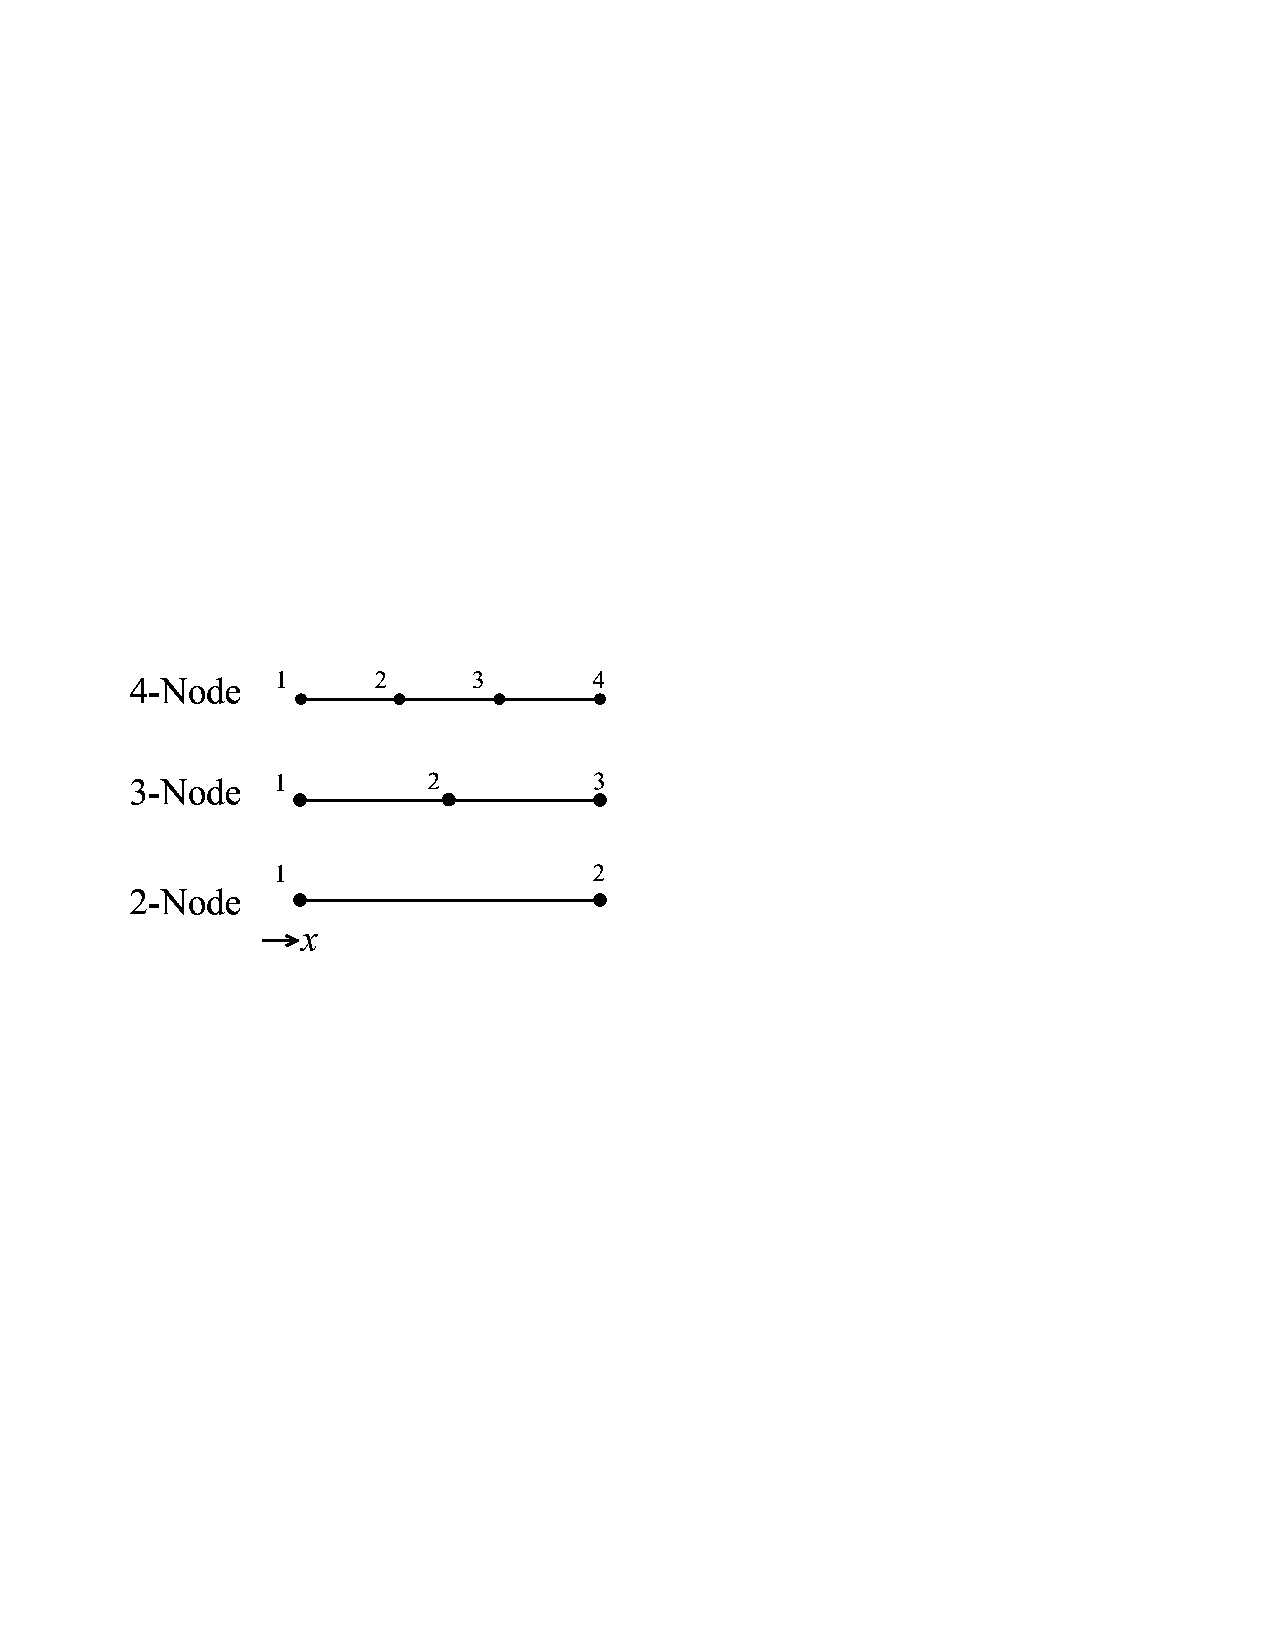
\includegraphics[trim=0.5in 4.5in 4.0in 4.0in, clip, height=1.6in]{fig/nodeordering1D.pdf}
\caption{Node ordering for 2-node, 3-node, and 4-node line elements}
\label{fig:NodeOrderingLine}
%\end{figure}
%\begin{figure}[htbp]
\begin{minipage}{\linewidth}
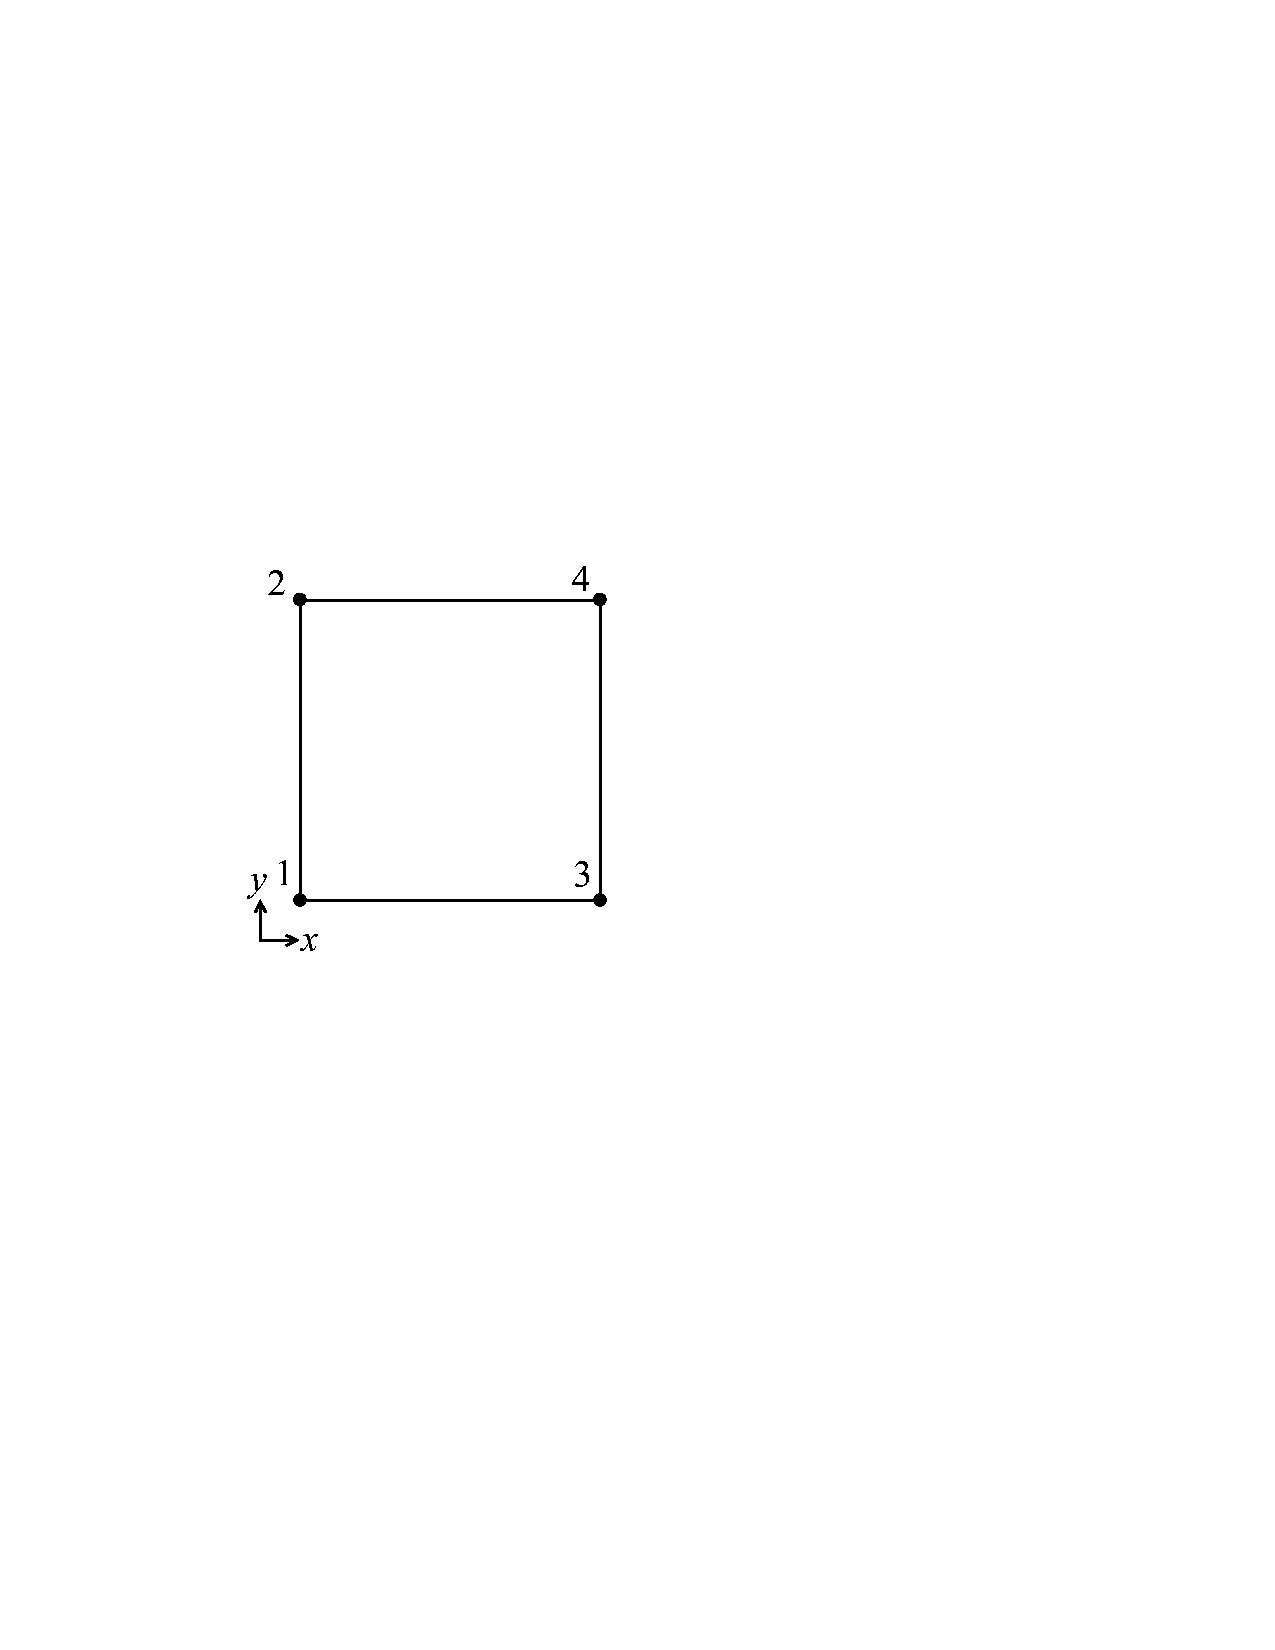
\includegraphics[trim=1.5in 4.5in 4.2in 3.5in, clip, height=2in]{fig/nodeordering2D_4.pdf}
\hfill
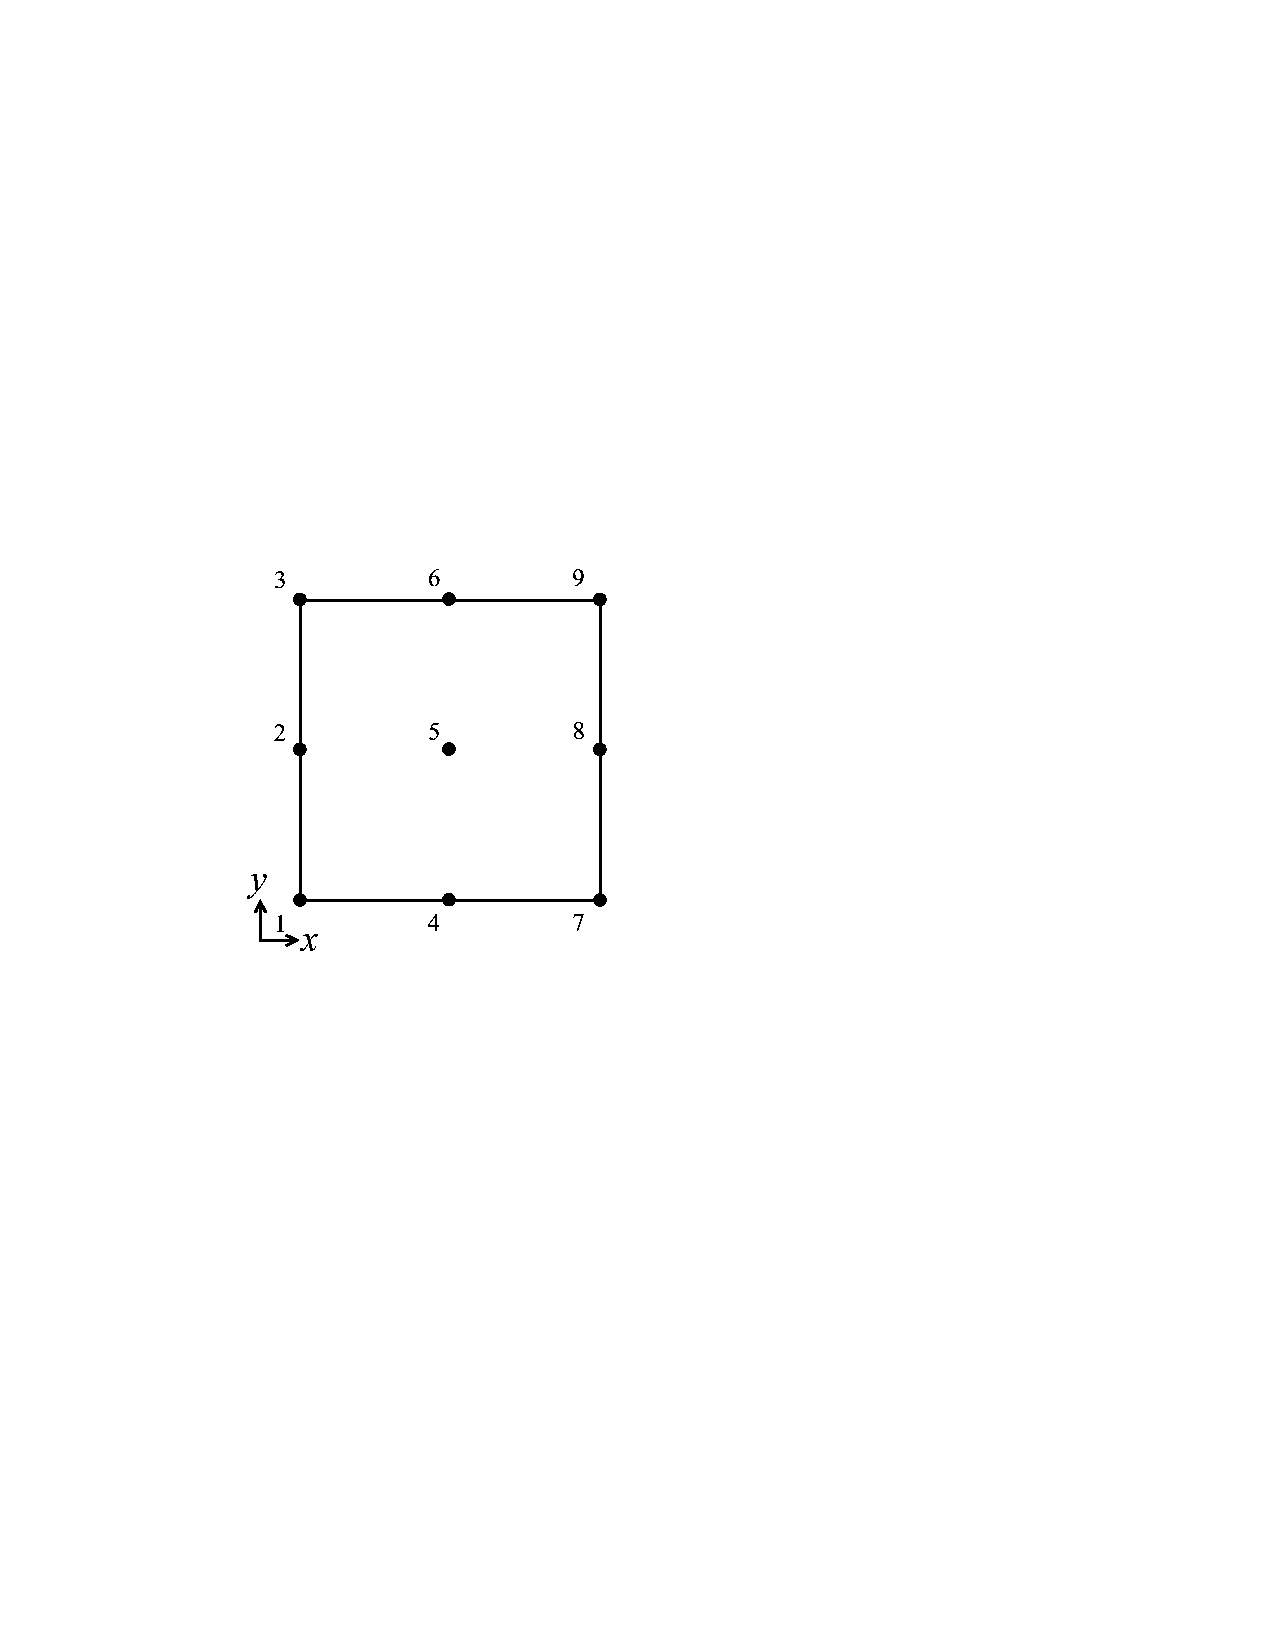
\includegraphics[trim=1.5in 4.5in 4.2in 3.5in, clip, height=2in]{fig/nodeordering2D_9.pdf}
\hfill
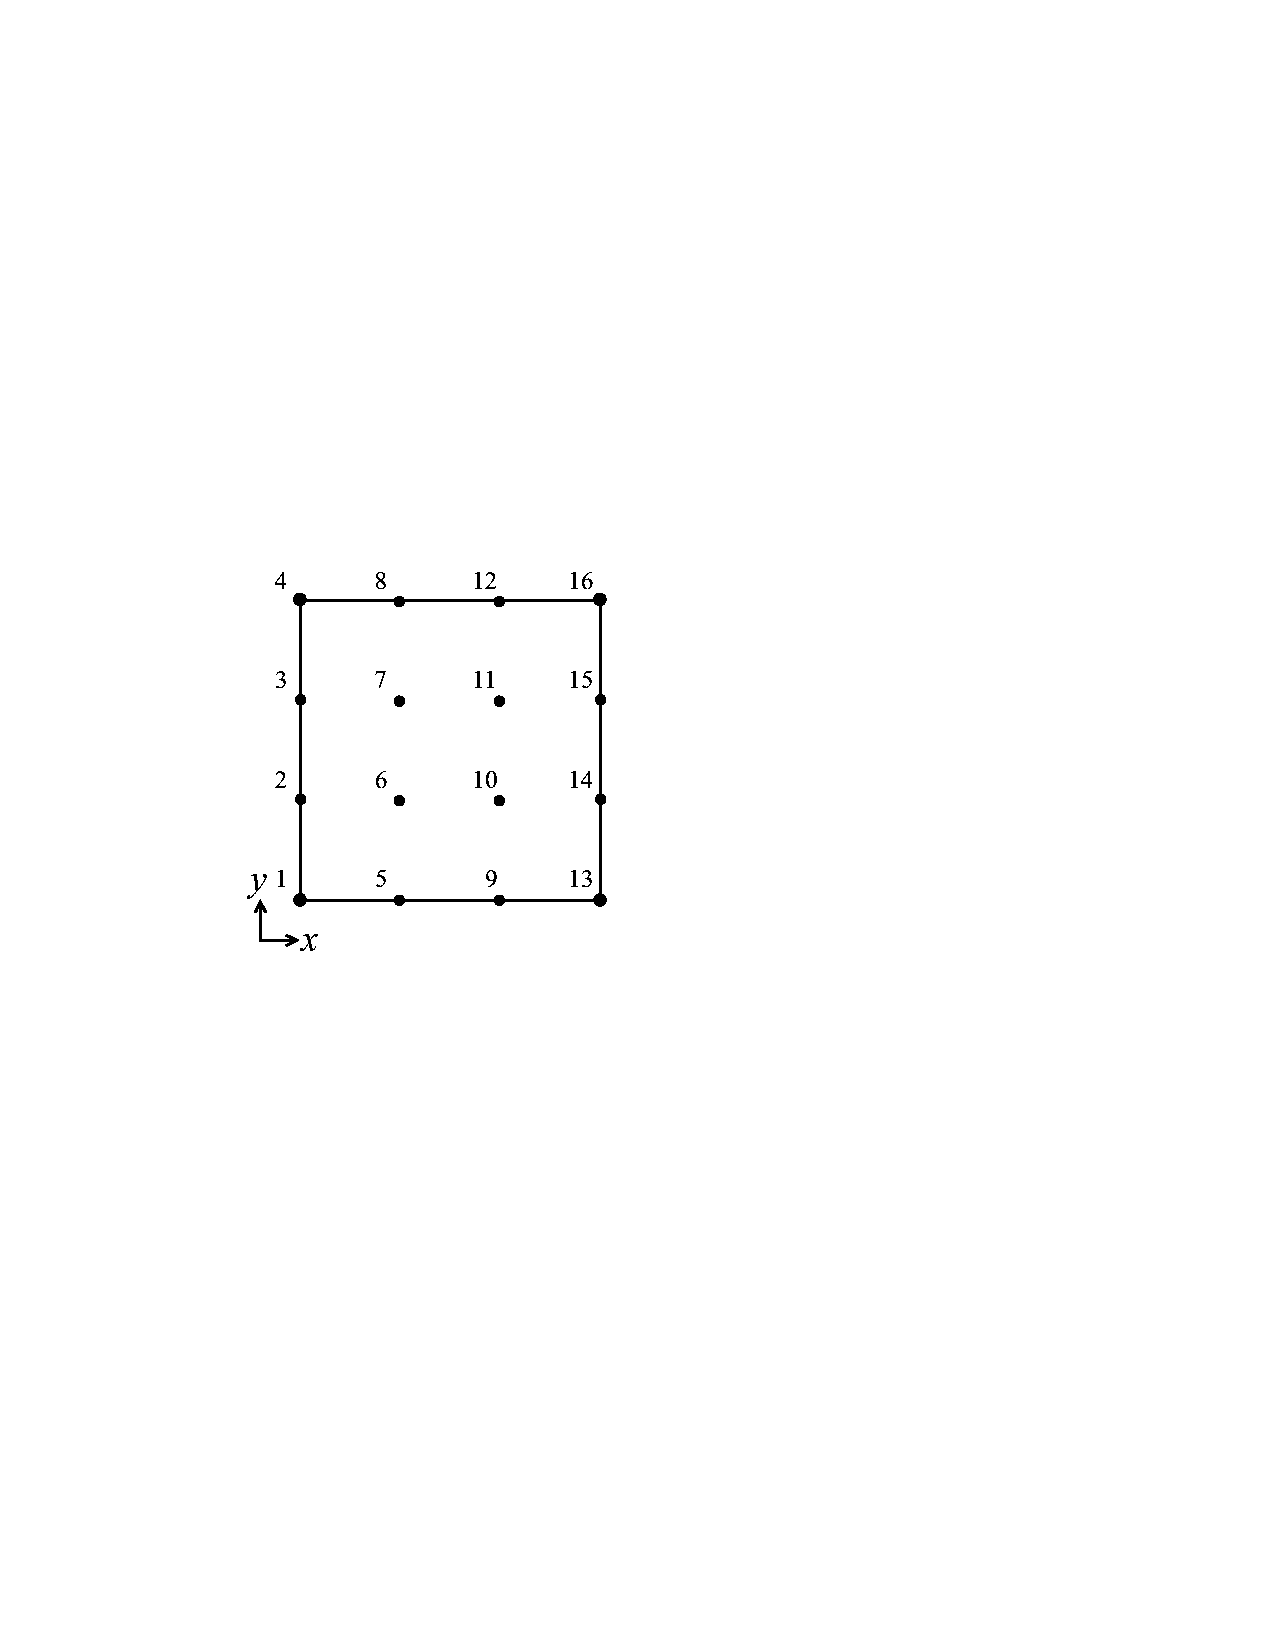
\includegraphics[trim=1.5in 4.5in 4.2in 3.5in, clip, height=2in]{fig/nodeordering2D_16.pdf}
\caption{Node ordering for 4-node, 9-node, and 16-node quads}
\label{fig:NodeOrderingQuad}
\end{minipage}
%\end{figure}
%\begin{figure}[htbp]
\centering
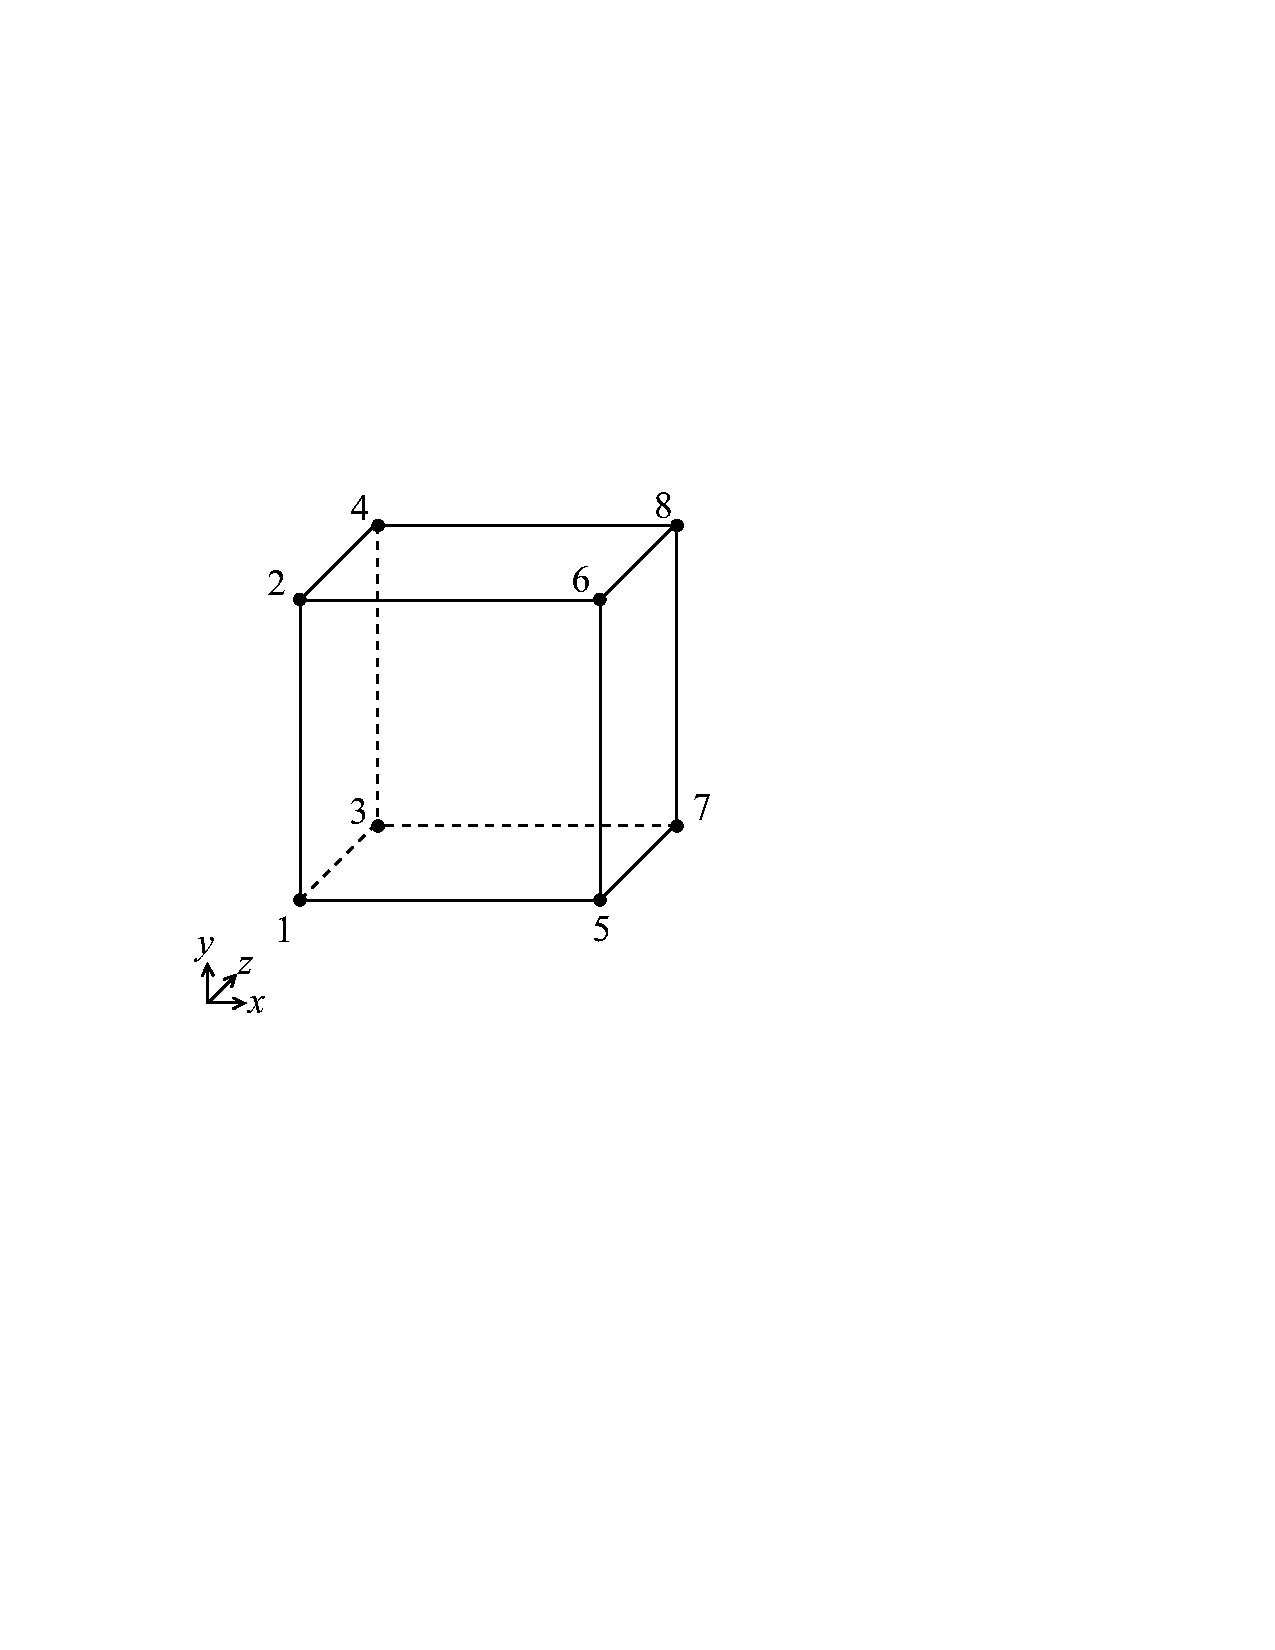
\includegraphics[trim=1.2in 4.2in 3.5in 3.0in, clip, height=2in]{fig/nodeordering3D_8.pdf}
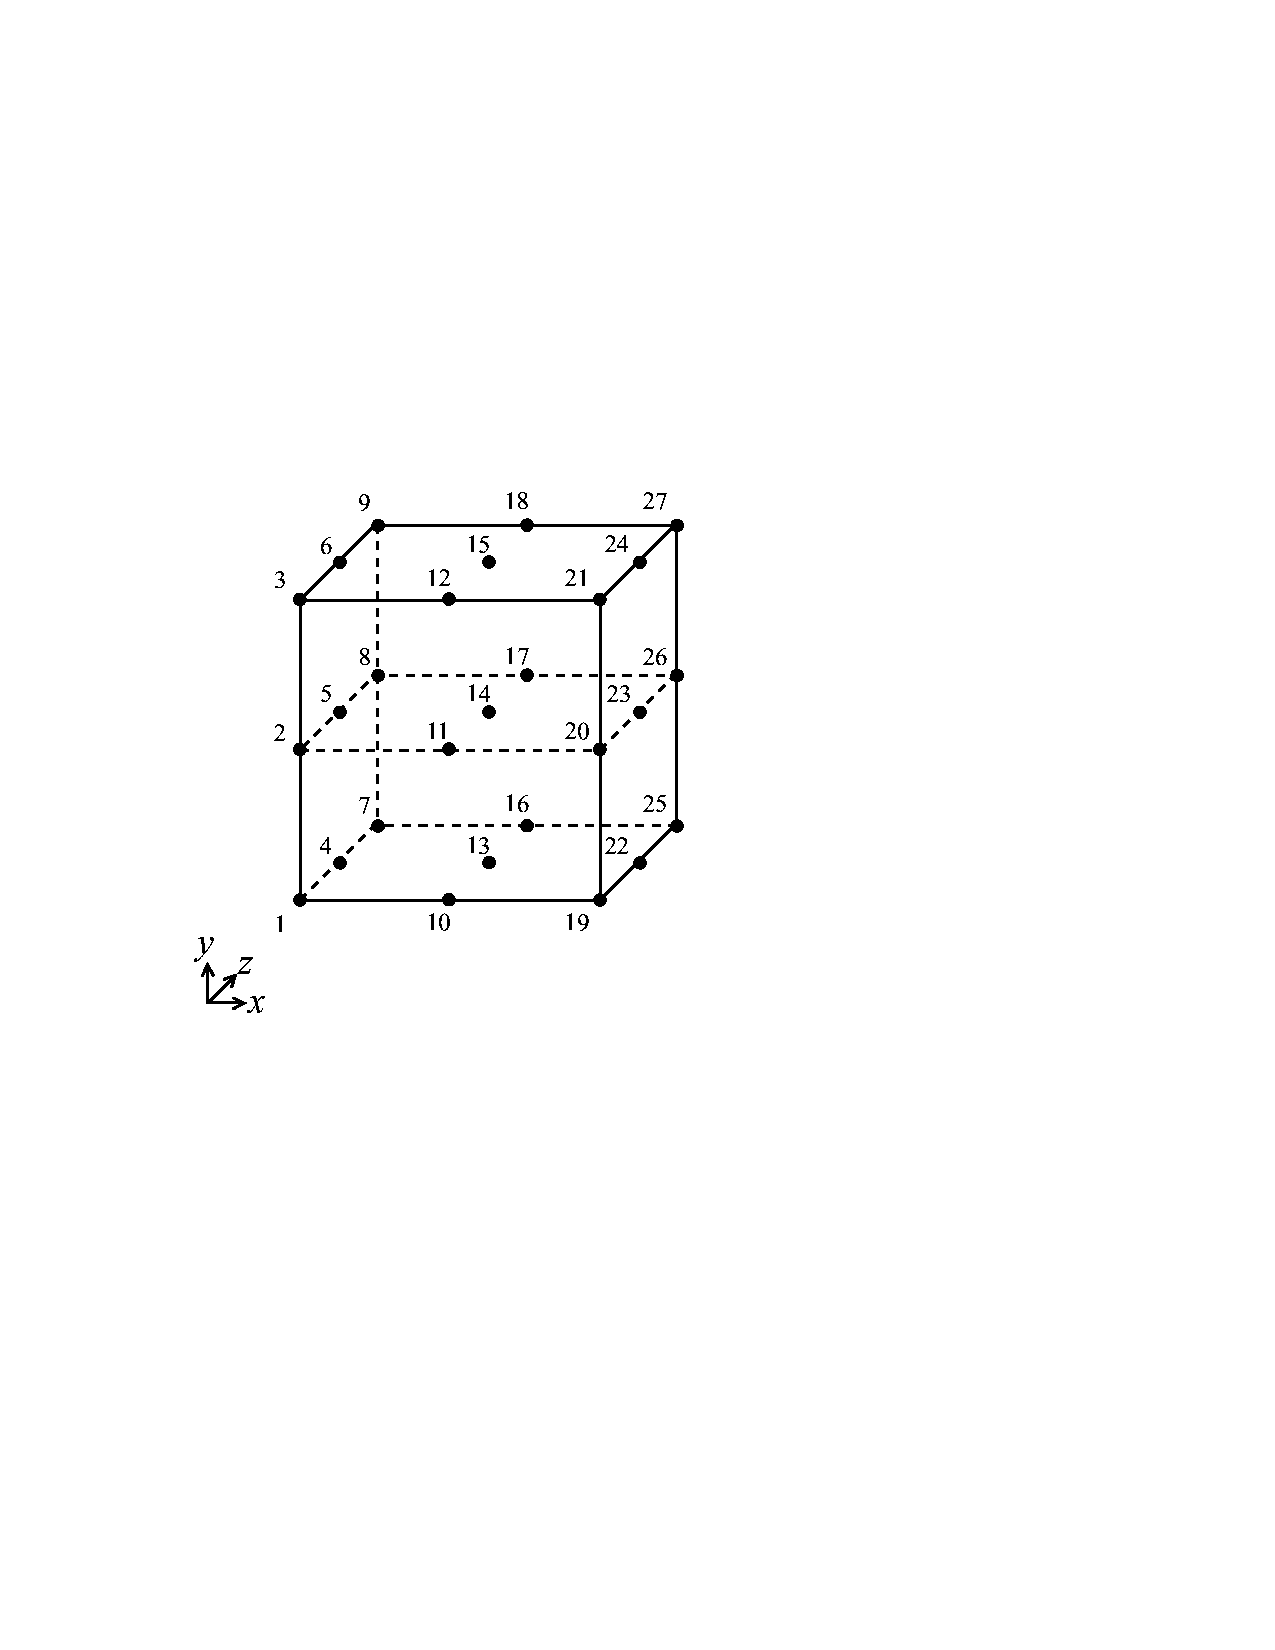
\includegraphics[trim=1.2in 4.2in 3.5in 3.0in, clip, height=2in]{fig/nodeordering3D_27.pdf}
\caption{Node ordering for 8-node and 27-node brick}
\label{fig:NodeOrderingBrick}
\end{figure}

\clearpage
\subsection{Block generators}
\label{section:BlockGenerators}
Thought the methods introduced above for adding nodes and 
elements are general, they can be tedious to use when defining
complicated geometry or for parametric mesh refinement analyses.
Mesh generation can be simplified by using the block generator
commands introduced in this section.

\subsubsection{Simple block generators}
\begin{codelist}
  \item[add\_block(x1,x2,nx,etype,order)]
    The \ttt{add\_block} methods allow you to add a Cartesian strip of
    elements.  This method takes two end points \ttt{x1,x2} and the 
    number of points along the edge (including end points), and constructs 
    a mesh of the strip $[x_{\min}, x_{\max}] \times$.  It is possible to
    remap the bricks later by directly manipulating the mesh \ttt{x}
    array.  Each element has a specified order, and the number of points
    along each edge should be one greater than a multiple of that order.
    Thus \ttt{nx} and \ttt{order} should satisfy the relation,
    \begin{eqnarray}
      \text{nx} &=& \text{order} \times
                    \text{(number of elements between end points)}
                    + 1 \nonumber
    \end{eqnarray}
    The case where we have 7 nodes (\ttt{nx=7}) with varying order of
    elements is shown in Figure \ref{fig:AddBlock1D}.
    \begin{figure}[htbp]
    \centering
    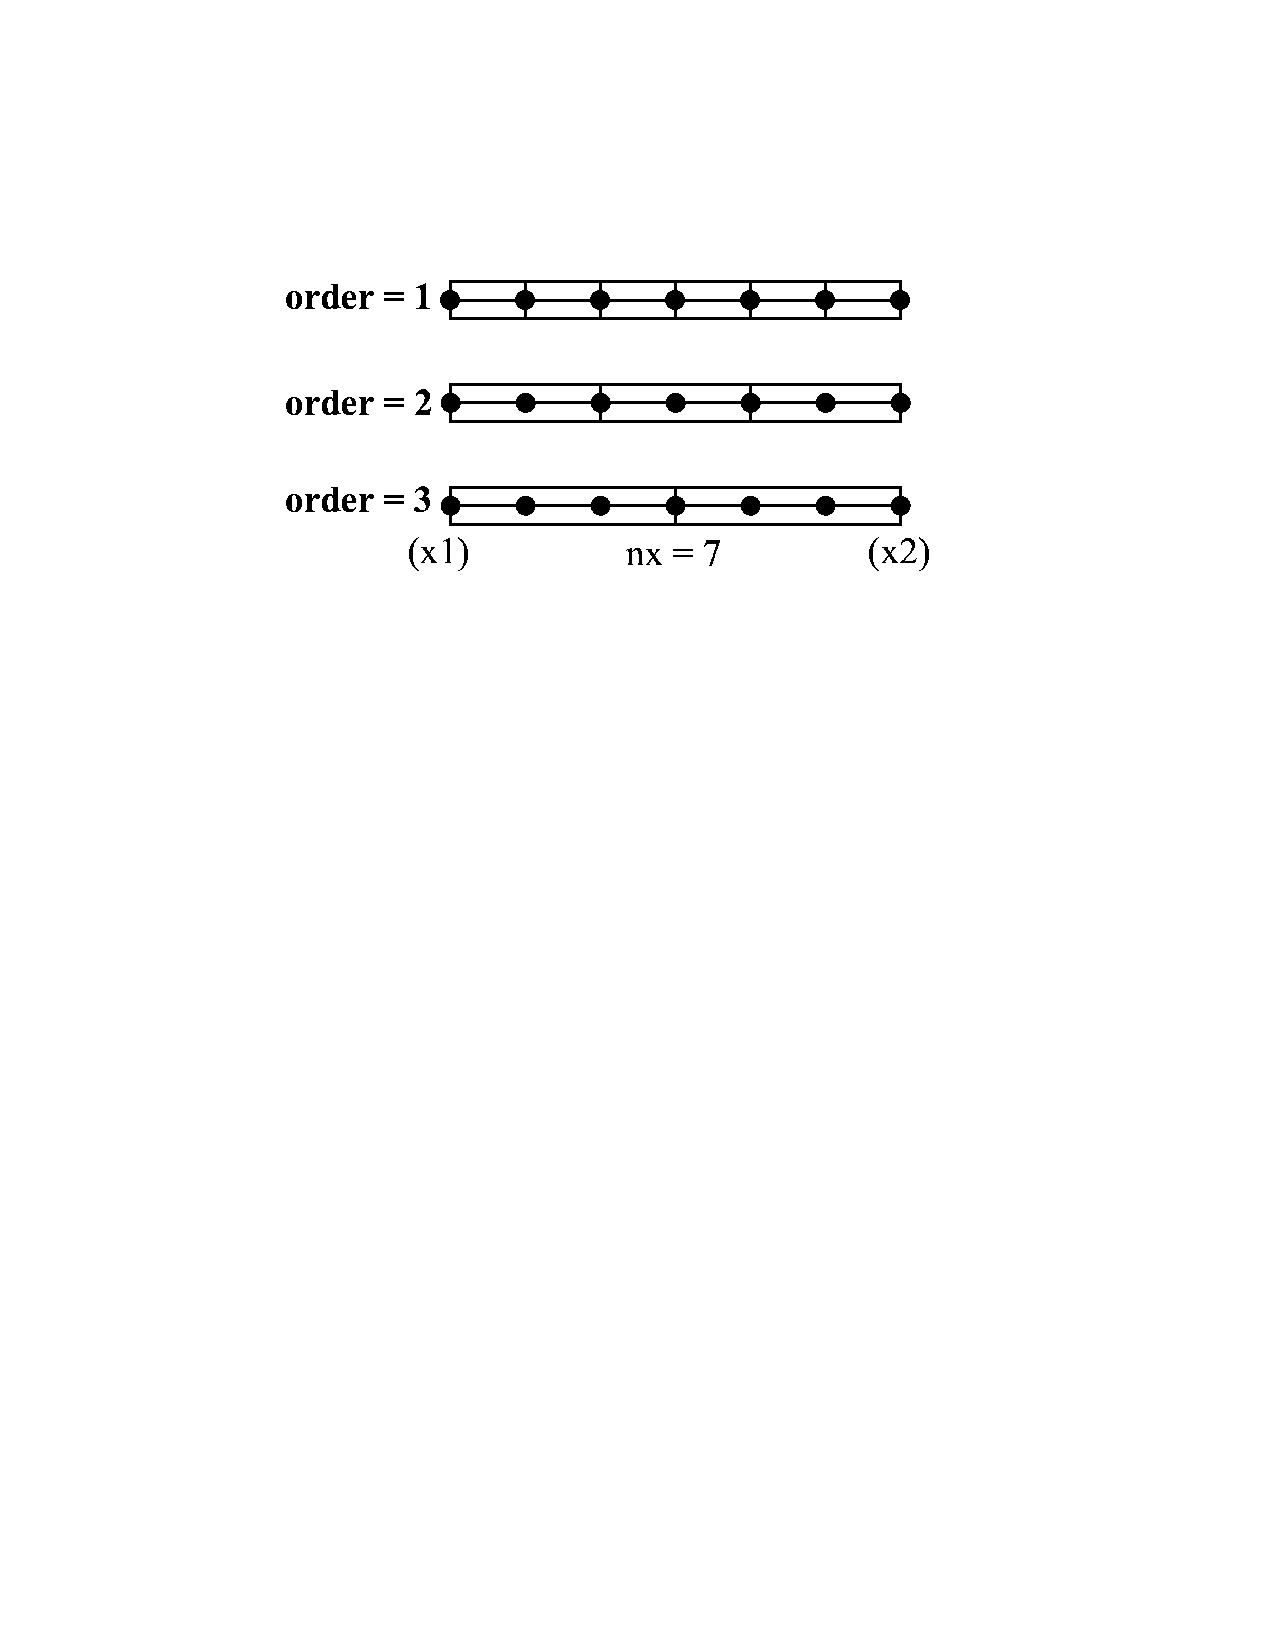
\includegraphics[trim=1.5in 6.5in 2.0in 1.6in, clip, height=2in]{fig/add_blocks1d.pdf}
    \caption{add\_block(x1,x2,nx=7,etype,order=1,2,3)}
    \label{fig:AddBlock1D}
    \end{figure}

\clearpage
  \item[add\_block(x1,y1,x2,y2,nx,ny,etype,order)]
    This is a 2D version of the \ttt{add\_block} generator.

    The case where we have 7 nodes (\ttt{nx=7}) by 3 nodes (\ttt{ny=3}) 
    with varying order of elements is shown in Figure \ref{fig:AddBlock2D}.
    We see here in this case that \ttt{nx,ny} both must satisfy the relation,
    \begin{eqnarray}
      \text{nx} &=& \text{order} \times
                    \text{(number of elements between end points)}
                    + 1 \nonumber \\
      \text{ny} &=& \text{order} \times
                    \text{(number of elements between end points)}
                    + 1 \nonumber
    \end{eqnarray}
    \begin{figure}[htbp]
    \centering
    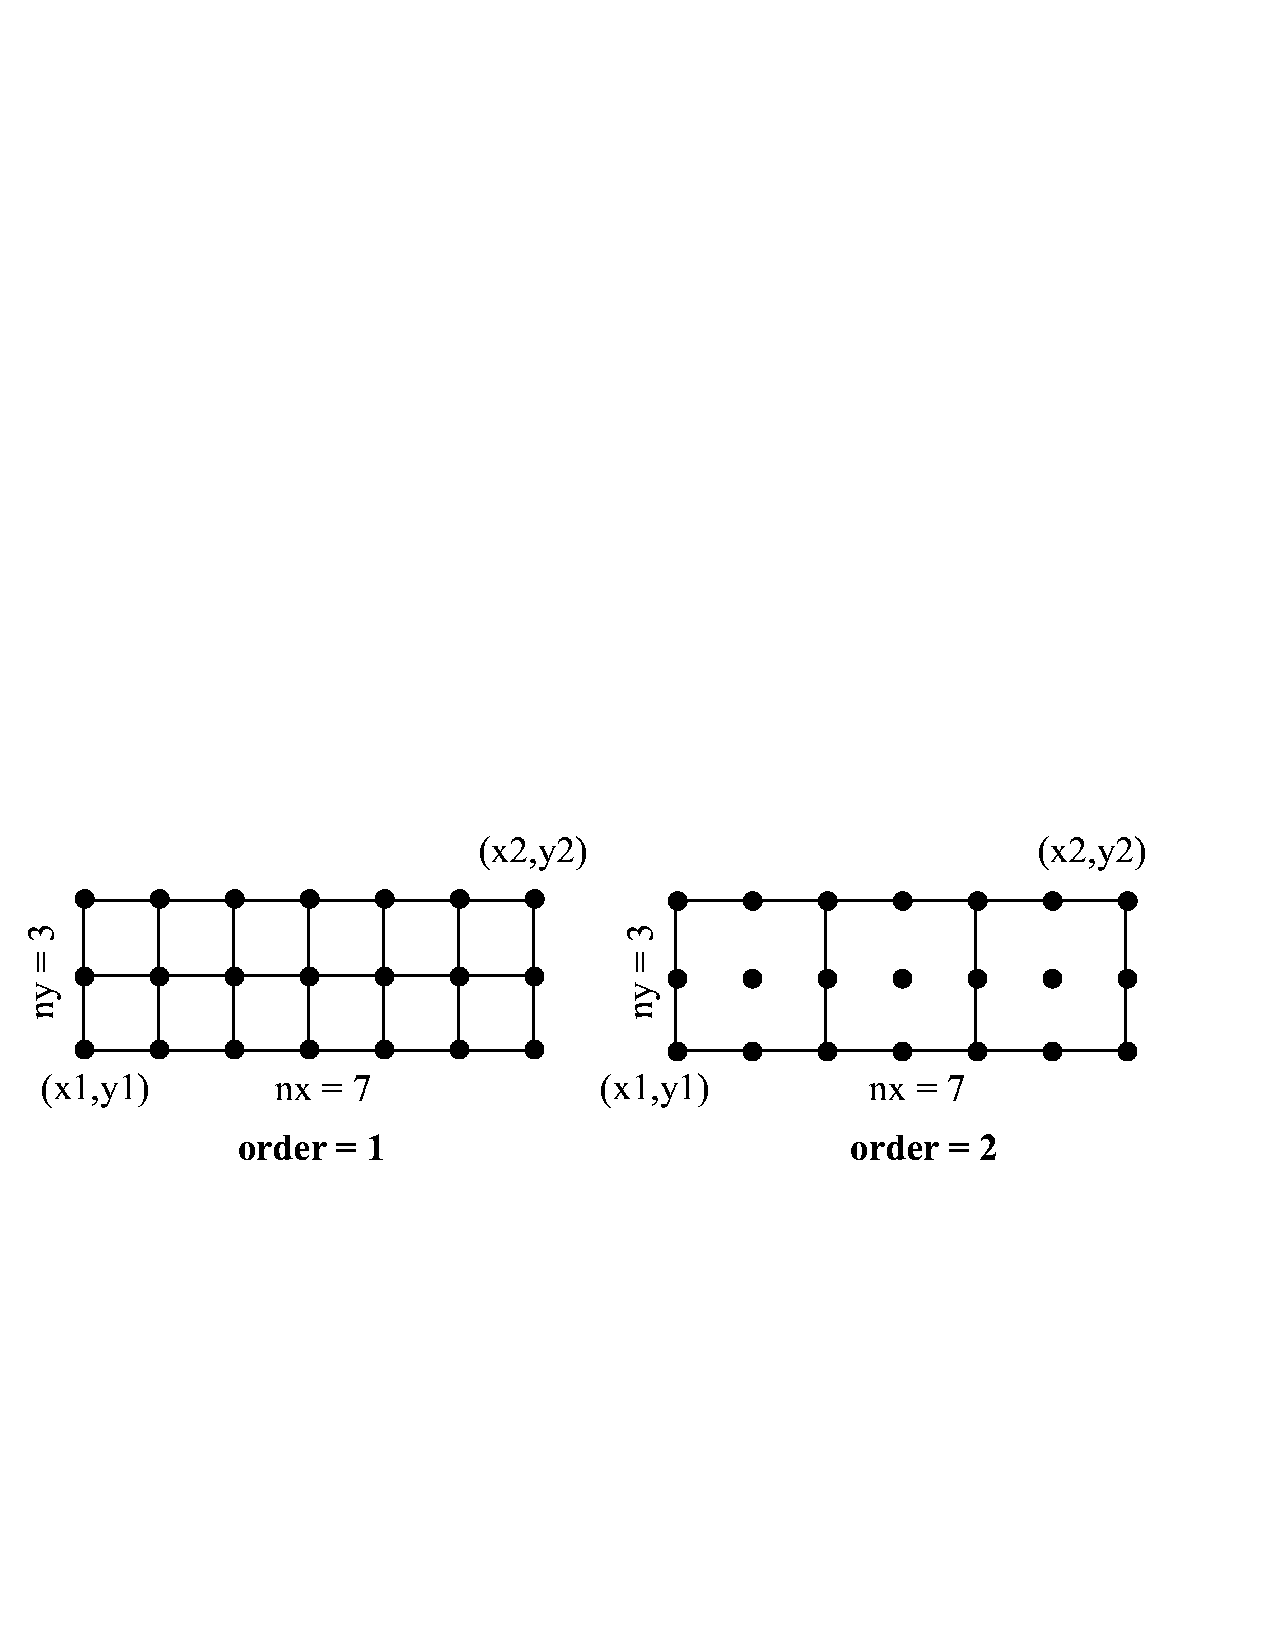
\includegraphics[trim=0.0in 3.0in 0.5in 5.3in, clip, height=1.7in]{fig/add_blocks2d.pdf}
    \caption{add\_block(x1,y1,x2,y2,nx=7,ny=3,etype,order=1,2)}
    \label{fig:AddBlock2D}
    \end{figure}

  \item[add\_block(x1,y1,z1,x2,y2,z2,nx,ny,nz,etype,order)]
    This is a 3D version of the \ttt{add\_block} generator. 
\end{codelist}

\clearpage
\subsubsection{Multiple block generators}
The block generators listed in this section can be understood 
as conducting multiple \ttt{add\_blocks} simultaneously.
This is done by passing an array of controls points along each edge,
and specifying the number of nodes along the edge between these
control points.
\begin{codelist}
  \item[blocks1dn(xlist,rlist,etype,order)]
    Creates a 1D strip of elements with specified nodes
    along the edge \ttt{xlist=\{x$_1$,...,x$_m$    \}}, and specified
    number of nodes along the edge between specified nodes
                   \ttt{rlist=\{r$_1$,...,r$_{m-1}$\}}.
    \ttt{r$_k$}($k=1,\ldots,m-1$) and \ttt{order} must satisfy the 
    relation stated in the generator \ttt{add\_block}. 

    The case where we have 3 control nodes, with 5 and 3 nodes along
    the edges between these nodes and varying order of elements, 
    is shown in Figure \ref{fig:Blocks1dn}.
    \begin{figure}[htbp]
    \centering
    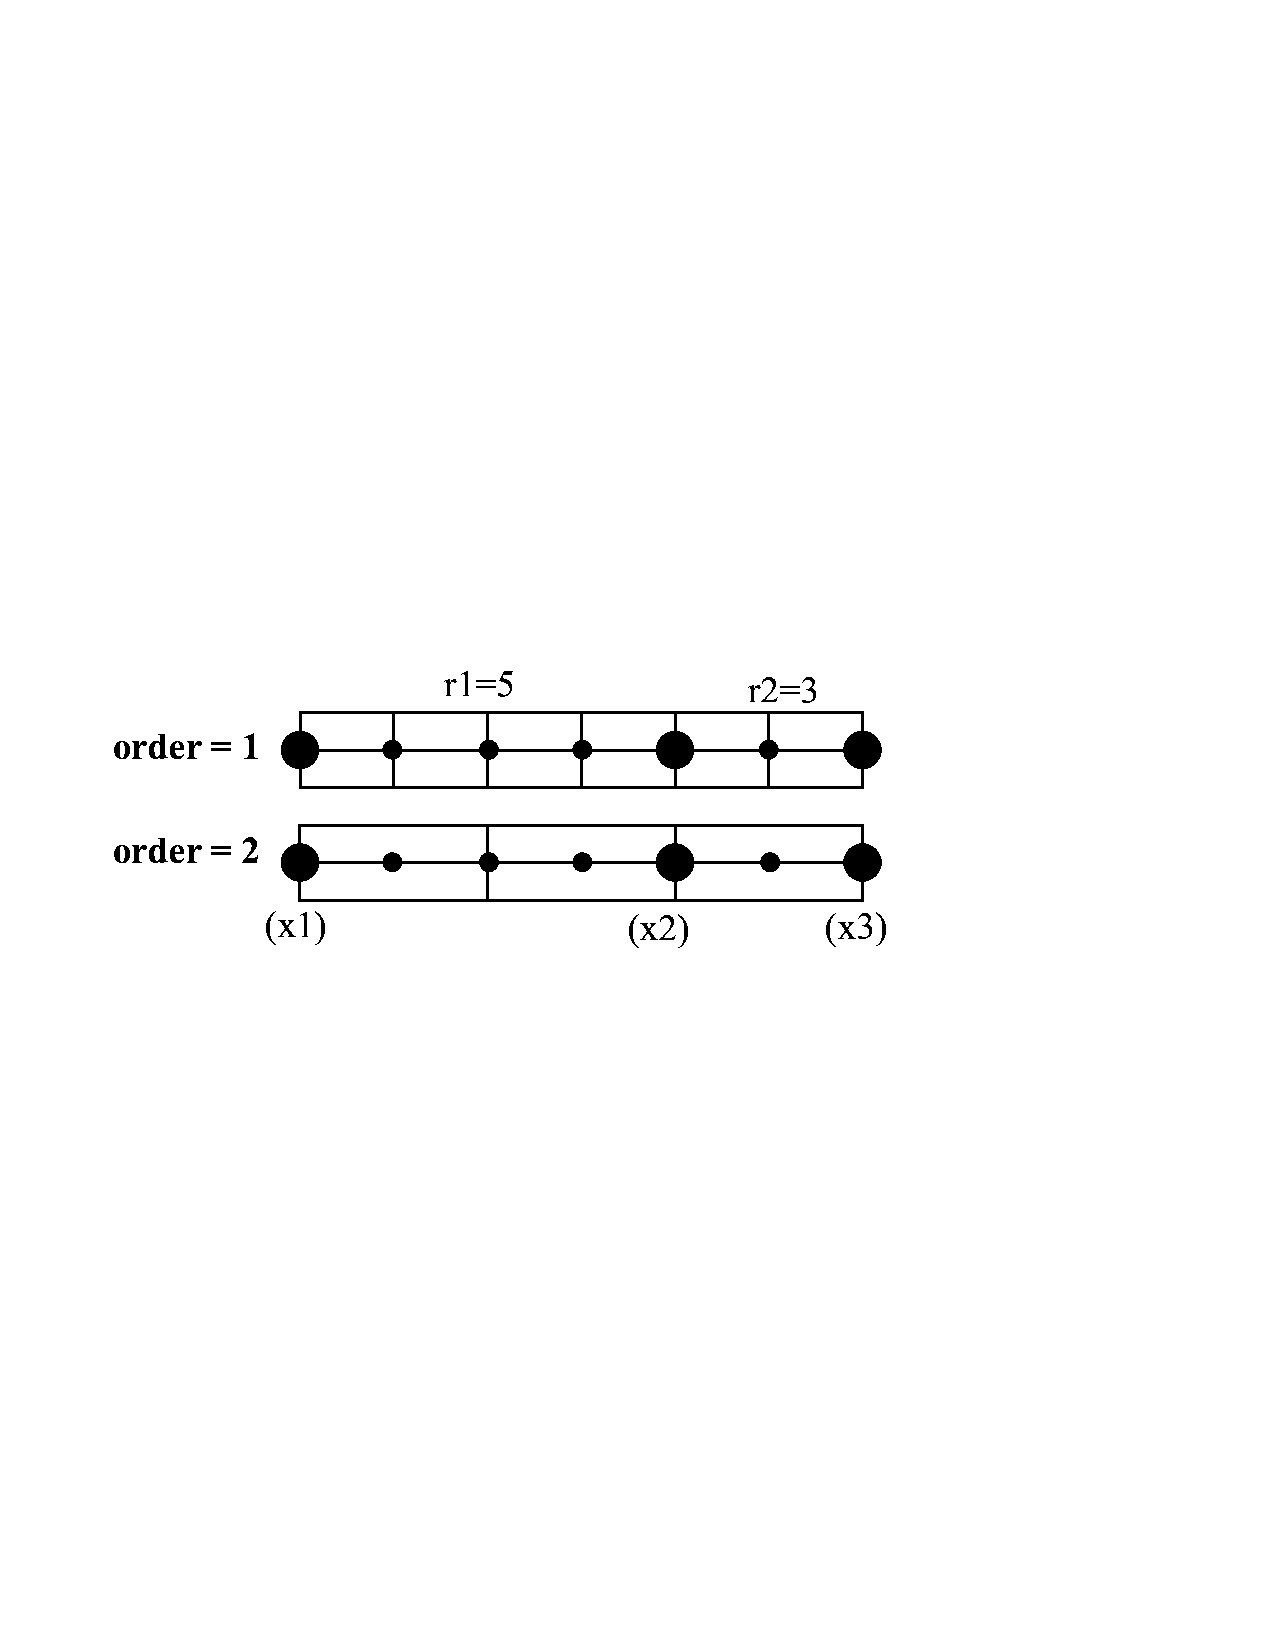
\includegraphics[trim=0.0in 4.5in 2.0in 4.2in, clip, height=1.5in]{fig/blocks1dn.pdf}
    \caption{blocks1dn(\{x1,x2,x3\},\{r1=5,r2=3\},etype,order=1,2)}
    \label{fig:Blocks1dn}
    \end{figure}

  \item[blocks2dn(xlist,rlist,ylist,slist,etype,order)]
    Creates a 2D block of elements with specified nodes
    along the edges 
    \ttt{xlist=\{x$_1$,...,x$_m$    \}}, 
    \ttt{ylist=\{y$_1$,...,y$_n$    \}}, and specified
    number of nodes along each edge between specified nodes
                   \ttt{rlist=\{r$_1$,...,r$_{m-1}$\}},
                   \ttt{slist=\{s$_1$,...,s$_{n-1}$\}}.
    Both \ttt{r$_k$}($k=1,\ldots,m-1$),\ttt{s$_k$}($k=1,\ldots,n-1$) 
    and \ttt{order} must satisfy the relation stated in the generator 
    \ttt{add\_block}. 

  \item[blocks3dn(xlist,rlist,ylist,slist,zlist,tlist,etype,order)]
    Creates a 3D block of elements with specified nodes
    along the edges 
    \ttt{xlist=\{x$_1$,...,x$_m$    \}}, 
    \ttt{ylist=\{y$_1$,...,y$_n$    \}}, 
    \ttt{zlist=\{z$_1$,...,z$_p$    \}}, and specified
    number of nodes along each edge between specified nodes
                   \ttt{rlist=\{r$_1$,...,r$_{m-1}$\}},
                   \ttt{slist=\{s$_1$,...,s$_{n-1}$\}},
                   \ttt{tlist=\{t$_1$,...,t$_{p-1}$\}}.
    Both \ttt{r$_k$}($k=1,\ldots,m-1$),\ttt{s$_k$}($k=1,\ldots,n-1$),
         \ttt{t$_k$}($k=1,\ldots,p-1$) 
    and \ttt{order} must satisfy the relation stated in the generator 
    \ttt{add\_block}. 
\end{codelist}

\newpage
\begin{codelist}
  \item[blocks1d(xlist,etype,order,dense1)]
    Creates a 1D strip of elements with specified nodes
    along the edge \ttt{xlist=\{x$_1$,...,x$_m$    \}}. Nodes
    are inserted between these nodes according to the parameter
    \ttt{dense1}, which specifies the approximate size of the
    element. The method will fit $r_k$ number of elements with
    \ttt{order} between the specified nodes, where $r_k~~(k=1,\ldots,m-1)$ 
    is defined by the equation,
    \begin{eqnarray}
    r_k &=& \text{order} * \text{ceil}\left(\frac{x_{k+1}-x_k}
                                                 {\text{dense1}}\right)
                         + 1~. \nonumber
    \end{eqnarray} 
    The function \text{ceil} rounds to the nearest integer towards infinity.
    If the parameter \ttt{order} or \ttt{dense1} is not specified, the
    method will look for a global variable with the name \ttt{order} and
    \ttt{dense}. If these are supplied, the method will execute with no
    error.  

    The case where we have 3 control nodes with specified \ttt{dense1} 
    is shown in Figure \ref{fig:Blocks1d}. Since the number of elements is
    specified by \ttt{dense1}, we can see that as we increase the order of 
    each element, the number of nodes increases. 
    \begin{figure}[htbp]
    \centering
    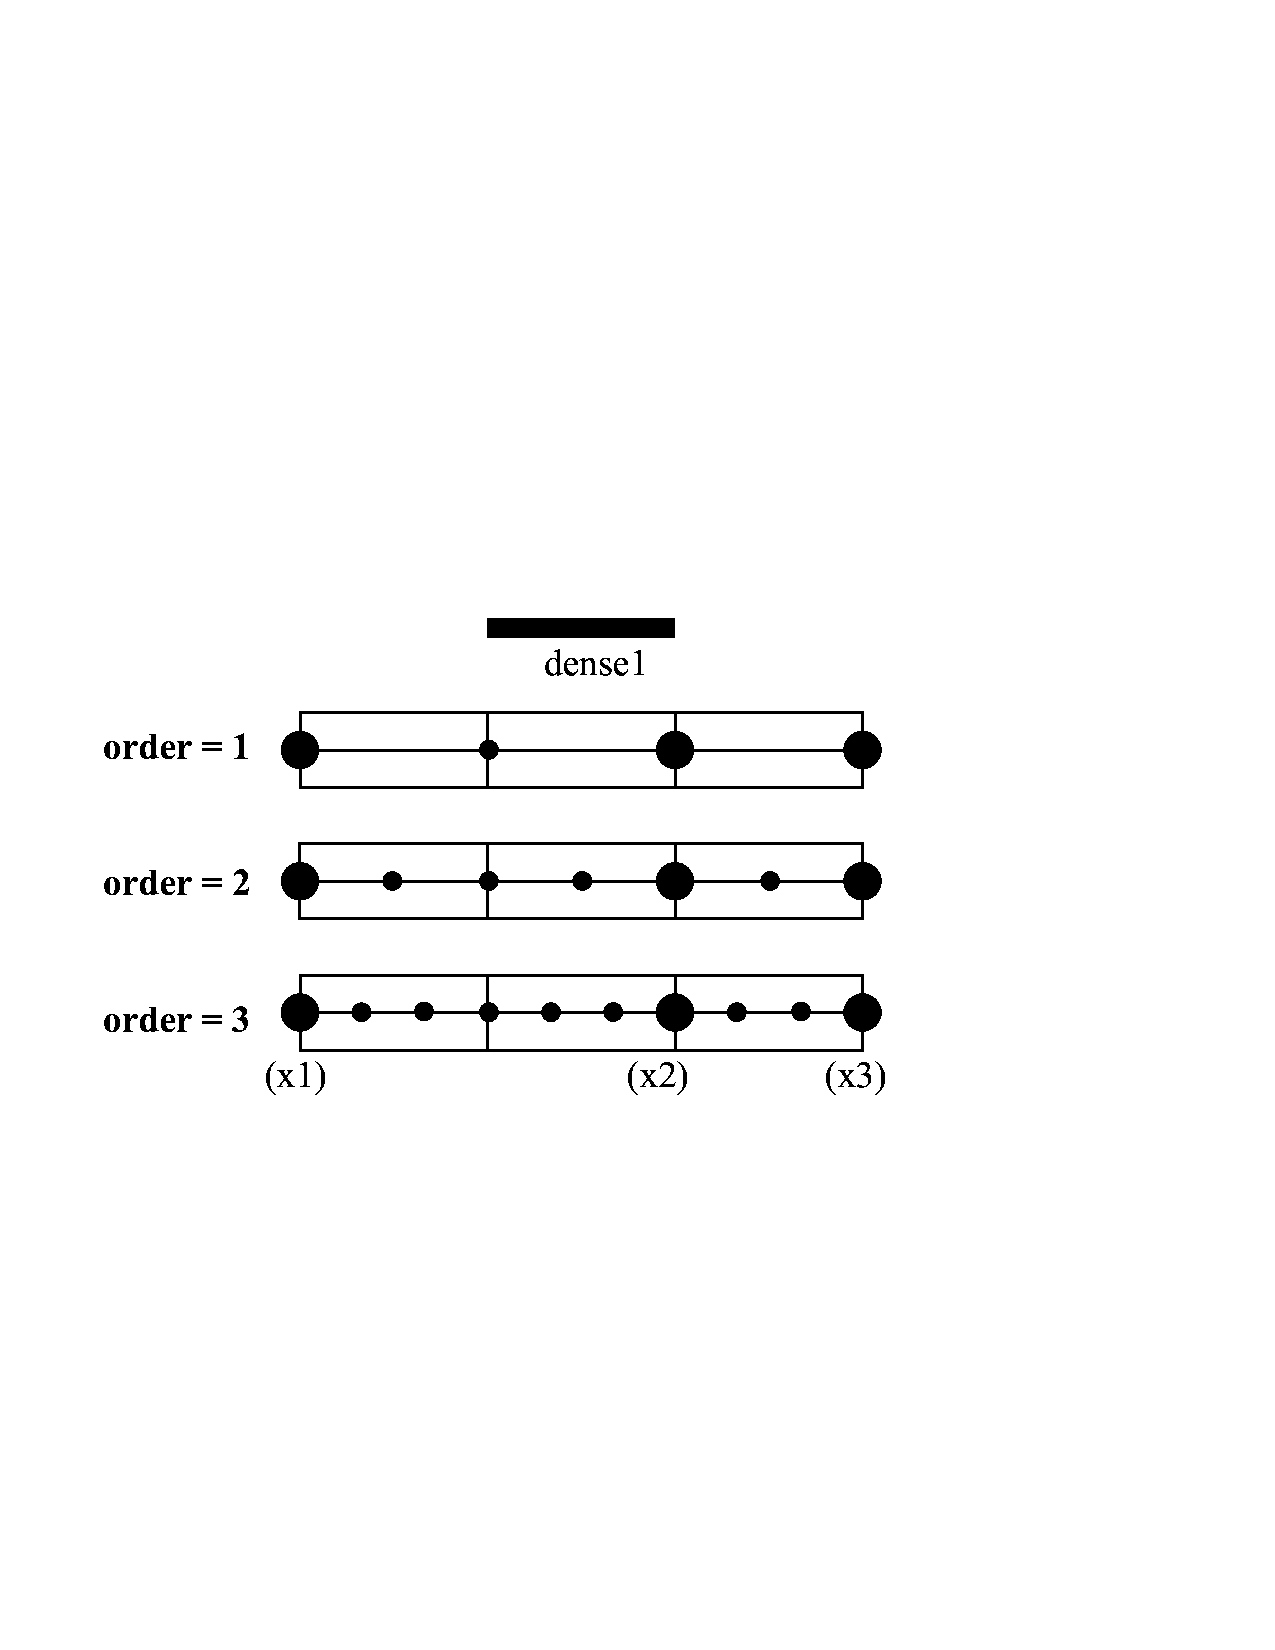
\includegraphics[trim=0.0in 3.5in 2.0in 4.0in, clip, height=1.7in]{fig/blocks1d.pdf}
    \caption{blocks1d(x=\{x1,x2,x3\},etype,order=1,2,3,dense1)}
    \label{fig:Blocks1d}
    \end{figure}
\end{codelist}
\clearpage
\begin{codelist} 
 \item[blocks2d(xlist,ylist,etype,order,dense1,dense2)]
    Creates a 2D block of elements with specified nodes
    along the edge 
    \ttt{xlist=\{x$_1$,...,x$_m$    \}},
    \ttt{ylist=\{y$_1$,...,y$_n$    \}}.
    Nodes are inserted between these nodes according to the parameter
    \ttt{dense1,dense2}, which specify the approximate size of the
    element. The method will fit $r_k$ number of elements in the $x$
    direction with \ttt{order} between the specified nodes, 
    and $s_k$ number of elements in the $y$
    direction with \ttt{order} between the specified nodes,
    where $r_k~~(k=1,\ldots,m-1)$, $s_k~~(k=1,\ldots,n-1)$ 
    is defined by the equation,
    \begin{eqnarray}
    r_k &=& \text{order} * \text{ceil}\left(\frac{x_{k+1}-x_k}
                                                 {\text{dense1}}\right)
                         + 1   \nonumber \\
    s_k &=& \text{order} * \text{ceil}\left(\frac{y_{k+1}-y_k}
                                                 {\text{dense2}}\right)
                         + 1~. \nonumber
    \end{eqnarray} 
    The function \text{ceil} rounds to the nearest integer towards infinity.
    If the parameter \ttt{order} or \ttt{dense1} \ttt{dense2} is not 
    specified, the method will look for a global variable with the name 
    \ttt{order} and \ttt{dense}. If these are supplied, the method will 
    assume \ttt{order = order }, \ttt{dense1 = dense}, and \ttt{dense2 = dense}
    and execute with no error.  

    The case where we have 3 control nodes along the $x$ direction and 
    2 control nodes along the $y$ direction with specified \ttt{dense1,dense2} 
    is shown in Figure \ref{fig:Blocks2d}. Since the number of elements is
    specified by \ttt{dense1,dense2}, we can see that as we increase the 
    order of each element, the number of nodes increases. 
    \begin{figure}[htbp]
    \centering
    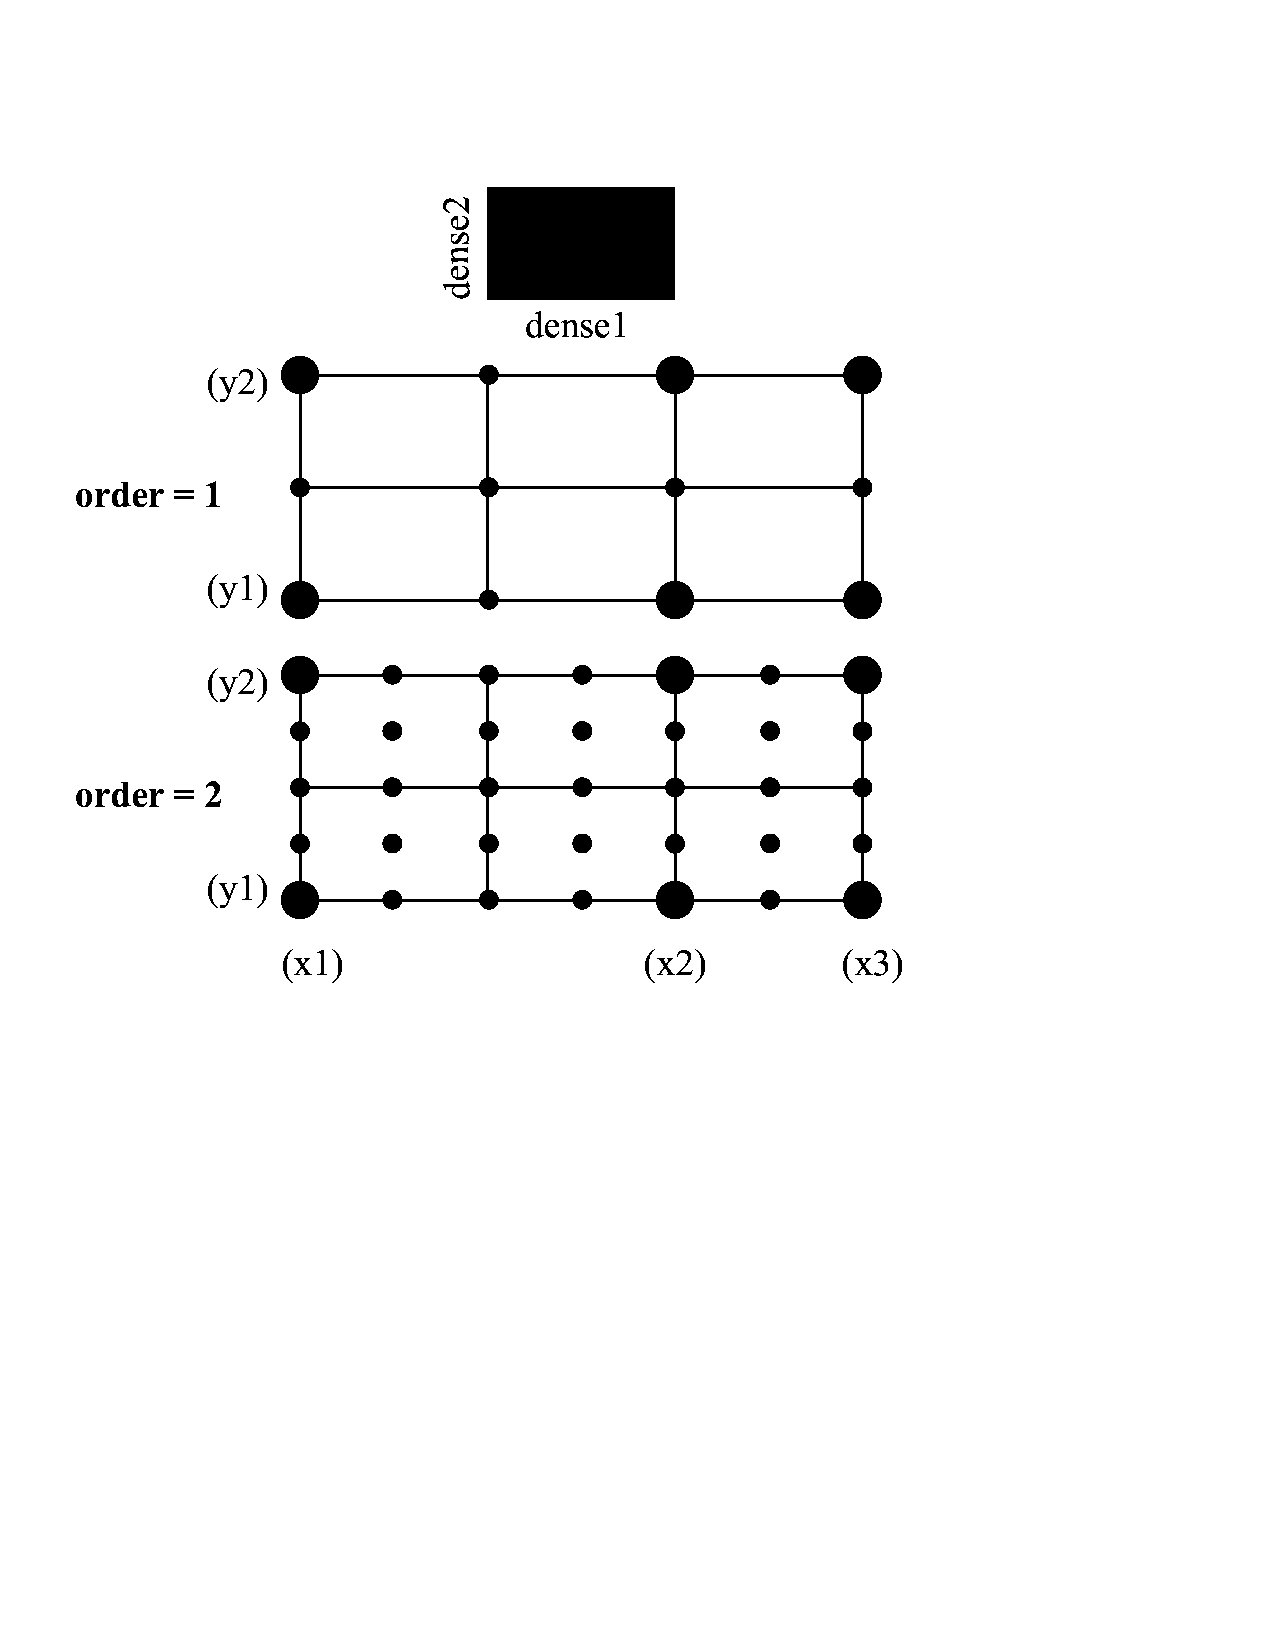
\includegraphics[trim=0.0in 4.5in 2.5in 1.0in, clip, height=2.5in]{fig/blocks2d.pdf}
    \caption{blocks2d(m=3,n=4,etype,order=1,func)}
    \caption{blocks2d(x=\{x1,x2,x3\},y=\{y1,y2\},etype,order=1,2,dense1,dense2)}
    \label{fig:Blocks2d}
    \end{figure}
  \item[blocks3d(xlist,ylist,zlist,etype,order,dense1,dense2,dense3)]
    Creates a 3D block of elements with specified nodes
    along the edge. 3D version of the function above. 

\end{codelist}

\clearpage
\subsubsection{Transformed block generation in Lua}
The block generators introduced in the previous two sections
are limitted to constructing square rectanglur mesh regions
which lacks flexibility. The generators presented in this 
section are versions of the \ttt{add\_block} command which can 
construct curved or non-rectangular blocks.
\begin{codelist}
  \item[add\_block\_shape(m,n,p,etype,order,pts)] 
    Creates a 3D (or 2D if \ttt{p} is omitted) quad block with node
    positions on $[-1,1]^ndm$ and transforms them using an isoparametric
    mapping with points specified in the \ttt{pts} array.  For
    example, for \ttt{pts = \{0,0, 0,1, 1,0, 1,1\}}, we would get a
    mesh for $[0,1]^2$.
    \ttt{m,n,p} and \ttt{order} must satisfy the relation stated in the 
    generator \ttt{add\_block}. 

    An example of a $[-1,1]^2$ region with 3 nodes along the x direction and
    4 nodes along the y direction mapped to a 4-noded polygon with 
    specified nodal points is presented in Figure \ref{fig:AddBlockShape}.
    \begin{figure}[htbp]
    \centering
    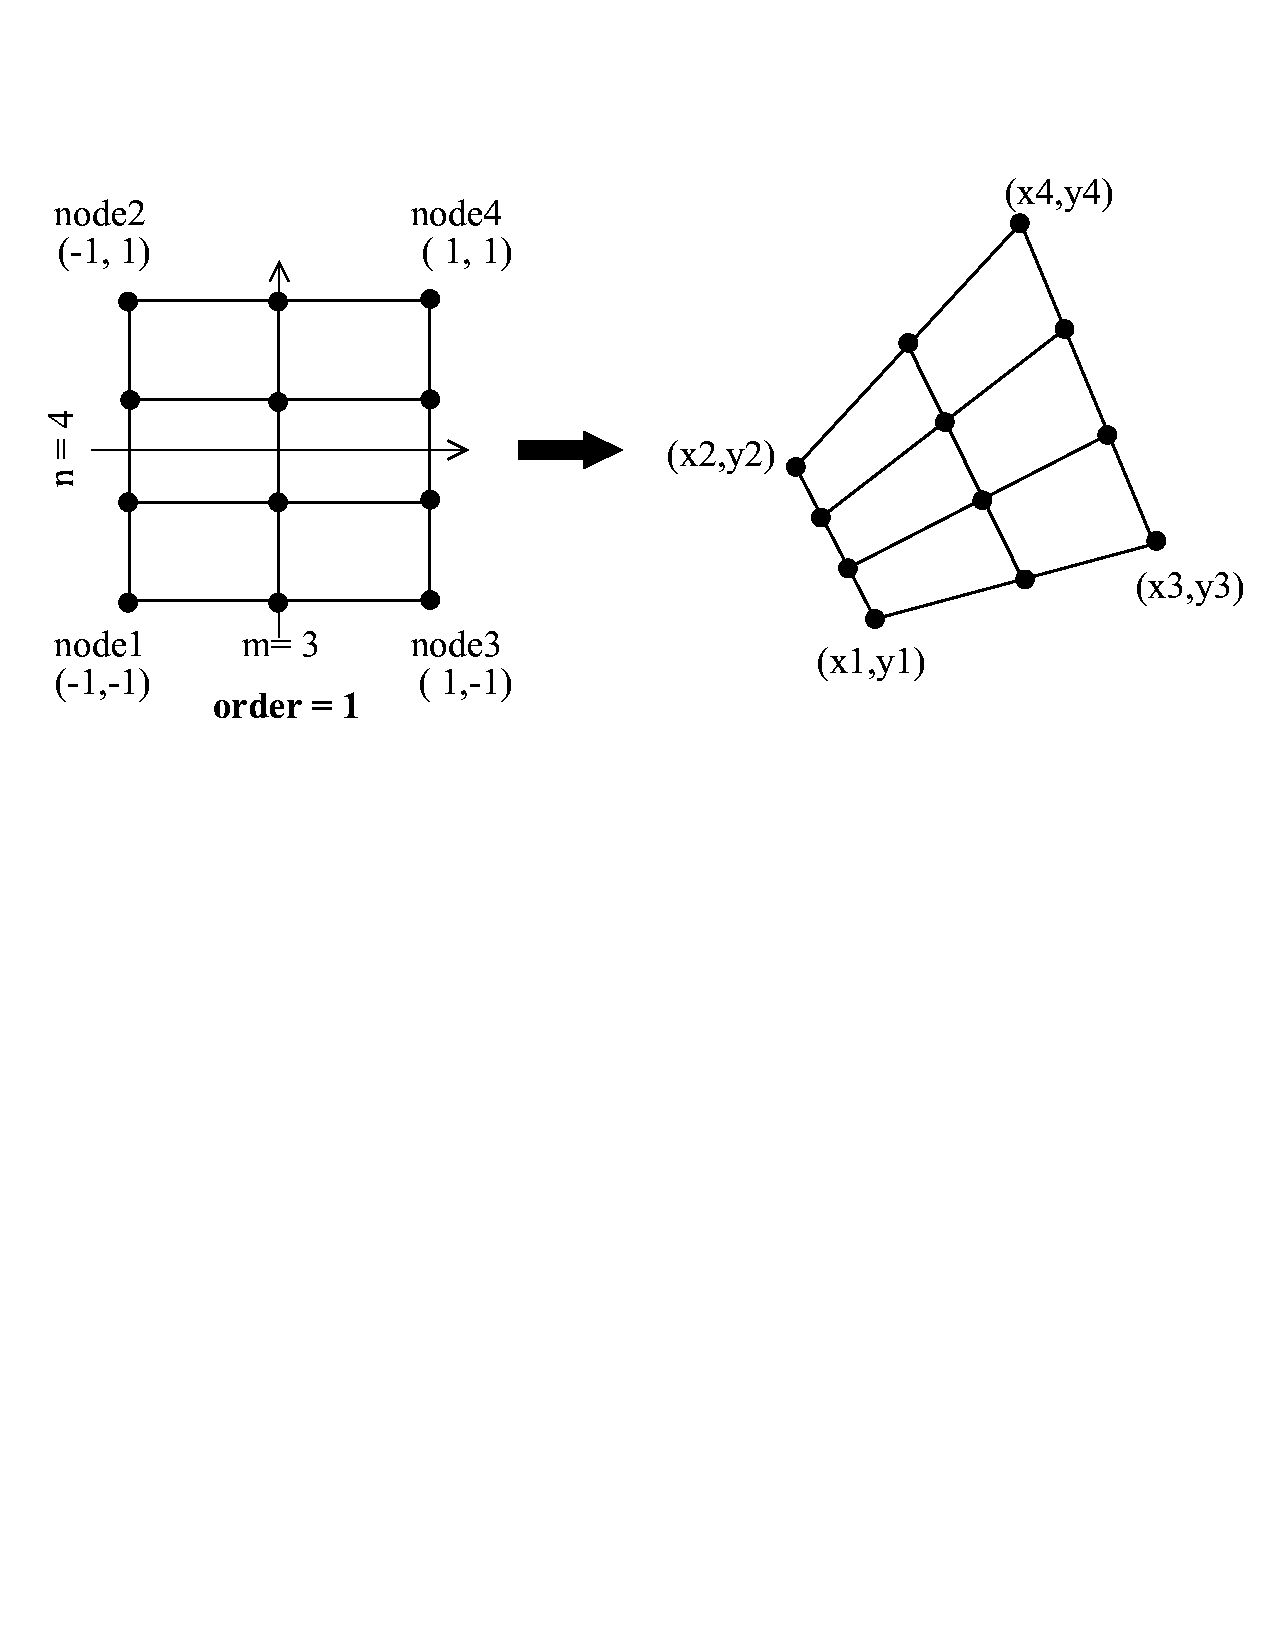
\includegraphics[trim=0.0in 5.5in 0.0in 1.0in, clip, height=1.7in]{fig/block_shape.pdf}
    \caption{add\_\_block\_shape(m=3,n=4,etype,order=1,pts)}
    \label{fig:AddBlockShape}
    \end{figure}

  \item[add\_block\_transform(m,n,p,etype,order,func)] 
    Creates a 3D (or 2D if \ttt{p} is omitted) quad block with node
    positions on $[-1,1]^ndm$ and transforms them using the specified
    function. The function \ttt{func} must have the following form for 2D,
    \begin{verbatim}
       function func(x,y)
         -- Compute mapped coordinates (new_x,new_y) from (x,y)
         return new_x,new_y
       end
    \end{verbatim}
    and for 3D,
    \begin{verbatim}
       function func(x,y,z)
         -- Compute mapped coordinates (new_x,new_y,new_z) from (x,y,z)
         return new_x,new_y,new_z
       end
    \end{verbatim}
    \ttt{m,n,p} and \ttt{order} must satisfy the relation stated in the 
    generator \ttt{add\_block}. 

    An example of a $[-1,1]^2$ region with 3 nodes along the x direction and
    4 nodes along the y direction mapped to a curved block according to a 
    polar mapping is presented in Figure \ref{fig:AddBlockTransform}.
    \begin{figure}[htbp]
    \centering
    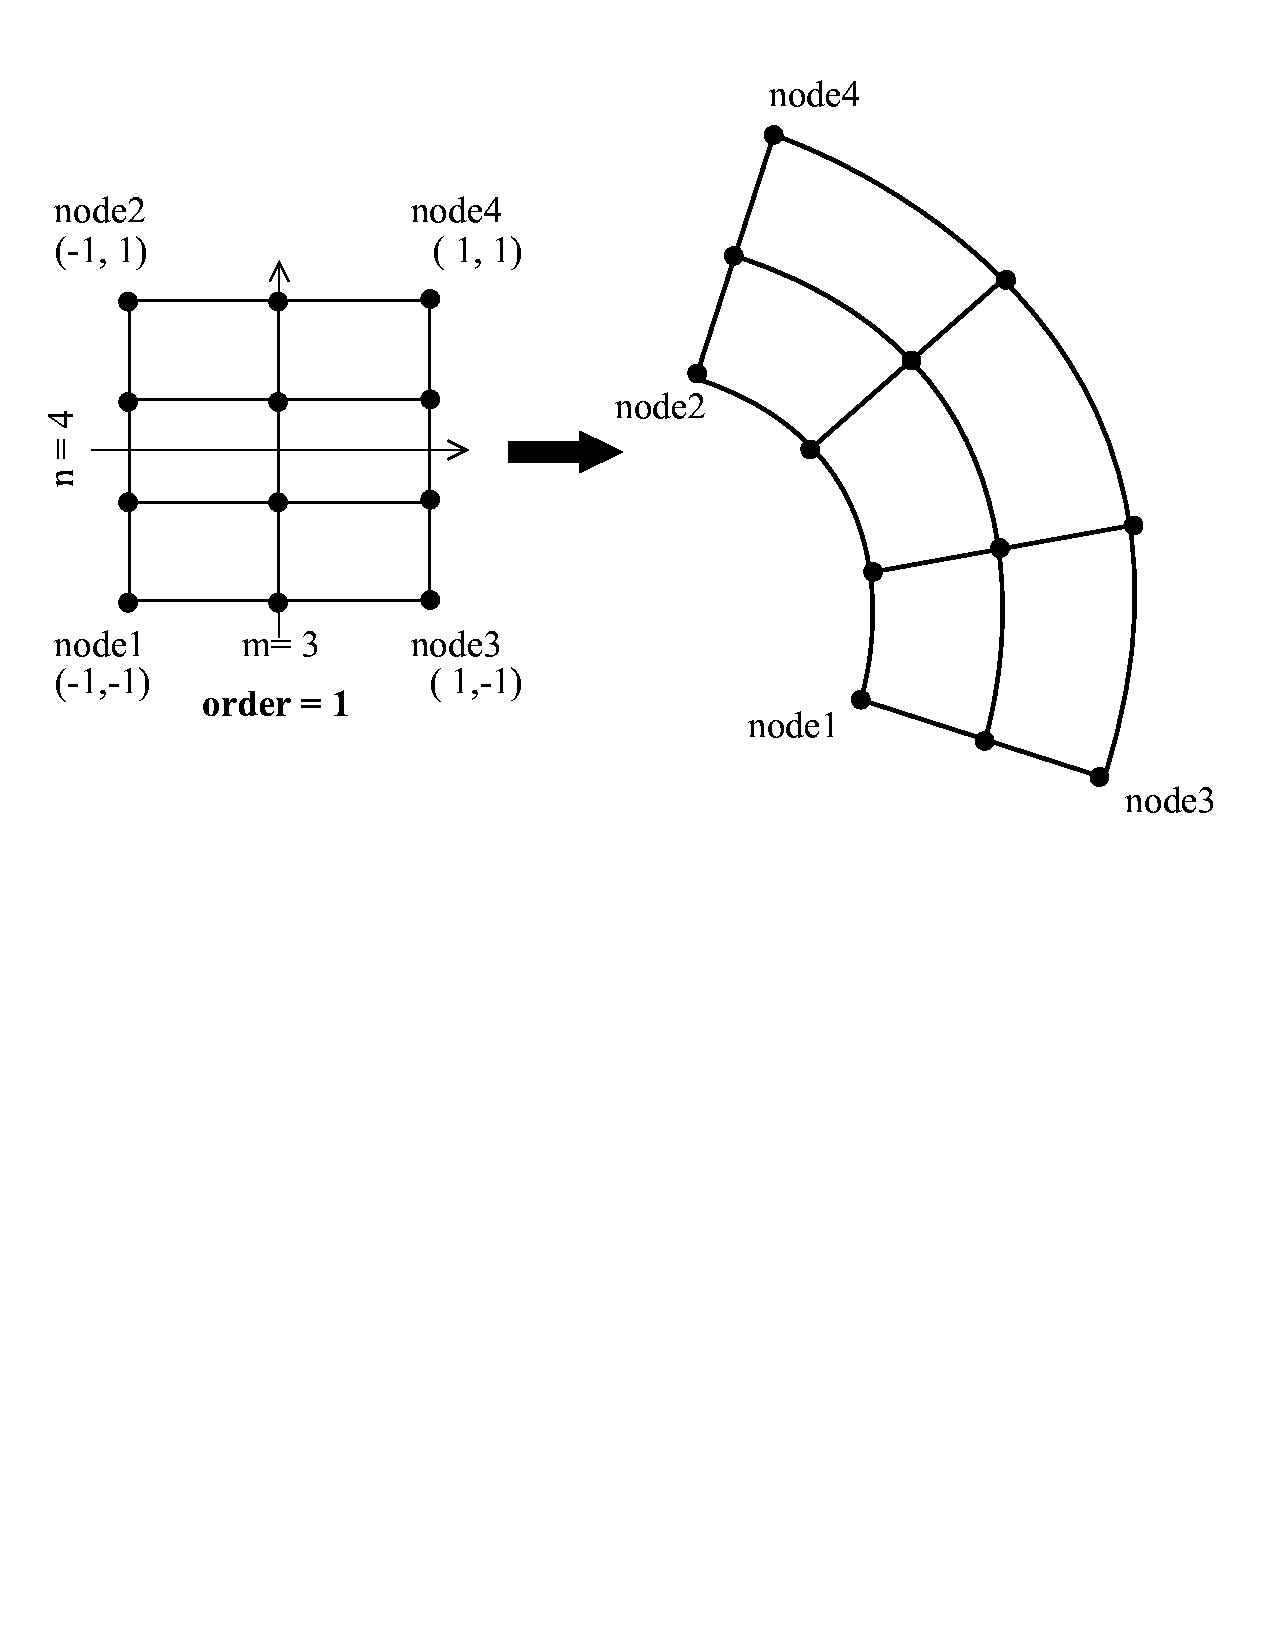
\includegraphics[trim=0.0in 5.5in 0.0in 0.5in, clip, height=1.7in]{fig/block_transform.pdf}
    \caption{add\_\_block\_transform(m=3,n=4,etype,order=1,func)}
    \label{fig:AddBlockTransform}
    \end{figure}

  \item[add\_curved\_block\_shape2d(m,n,etype,order,pts,curv)]
    Creates a 2D quad block with nodes positions on $[-1,1]^2$, 
    \ttt{m} node points along the $x$ direction and \ttt{n} node
    points along the $y$ direction, both including edge points. 
    \ttt{m,n} and \ttt{order} must satisfy the relation stated in
    the generator \ttt{add\_block}. The nodes on the corner of the 
    quad block are mapped to the 4 node points stored in the table
    \ttt{pts=\{x1,y1,x2,y2,x3,y3,x4,y4\}}. The table 
    \ttt{curv=\{curv1,curv2,curv3,curv4\}} contains the curvature
    on each edge, positive values specifying outward curvature and 
    negative values inward curvature.
    \ttt{m,n} and \ttt{order} must satisfy the relation stated in the 
    generator \ttt{add\_block}. 

    An example of a $[-1,1]^2$ region with 3 nodes along the x direction and
    4 nodes along the y direction mapped to a curved block with 4 control
    nodes and various curvatures on the edges is presented in 
    Figure \ref{fig:AddCurvedBlockShape2D}.
    \begin{figure}[htbp]
    \centering
    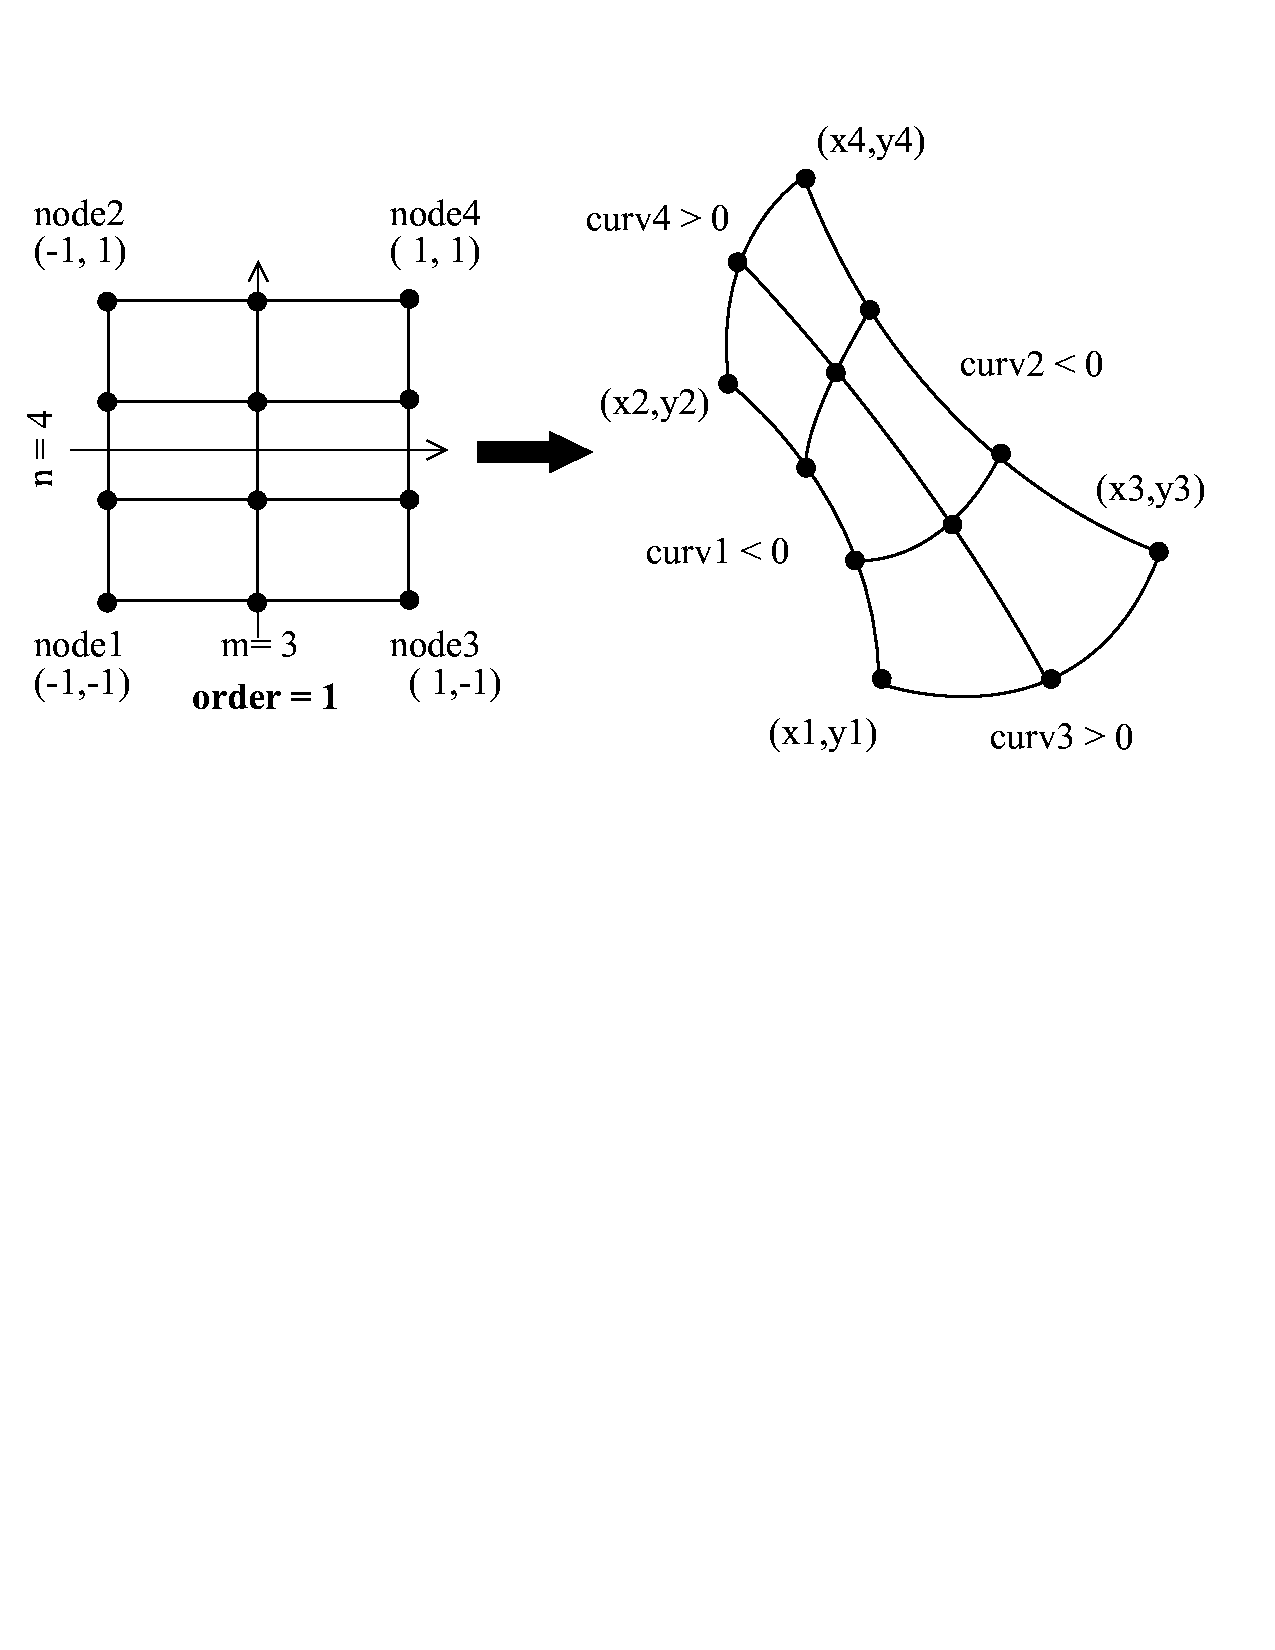
\includegraphics[trim=0.0in 5.5in 0.0in 0.5in, clip, height=1.7in]{fig/block_curved_block.pdf}
    \caption{add\_curved\_block\_shape2d(m=3,n=4,etype,order=1,pts,curv)}
    \label{fig:AddCurvedBlockShape2D}
    \end{figure}
\end{codelist}

\clearpage
\subsection{Tie command}
The mesh class also has a \ttt{tie} method which ``merges'' nodes
which are close to each other.  
\begin{codelist}
  \item[tie(tol)] The \ttt{tie} method takes a
  tolerance \ttt{tol} to try to tie nodes together. If this argument isn't
  specified, the method will look for a global parameter named \ttt{meshtol}.
  When this is given, the method will execute without error.
  If \ttt{tie} finds that nodes $i$ and $j$ in the specified range are
  within the given tolerance of each other, the \ttt{ix} array is
  rewritten so that references to either $i$ or $j$ become references to
  $\min(i,j)$.
\end{codelist}

The \ttt{tie} method acts as though the relation ``node $i$ is
within the tolerance of node $j$'' were an equivalence relation.  But
while this relation is reflexive and symmetric, it does \emph{not}
have to be transitive for general meshes: that is, if $x_i$, $x_j$,
and $x_k$ are three node positions, you might have
\[
  \|x_i - x_j\| < \mathrm{tol} \mbox{ and }
  \|x_j - x_k\| < \mathrm{tol} \mbox{ and }
  \|x_i - x_k\| > \mathrm{tol}.
\]
The behavior of the \ttt{tie} algorithm is undefined in this case.
Make sure it does not happen in your mesh.

\devnote{The right thing to do here is to make the semantics explicit
  (by using the transitive closure of the above relationship, for
  instance) and warn the user if there were any places where the
  behavior of the tie command is not obvious.}

\subsection{Applying boundary conditions}
There are three types of boundary conditions that can be set.
\begin{itemize}
\item Nodal boundary conditions: These are set on the degrees of 
      freedom of each node in the mesh.
\item Global variable boundary conditions: These are set on the 
      global degrees of freedom that can be set. (See section on
      global variables for details).
\item Element variable boundary conditions: These are set on the
      variables that pertain to a specific element. 
\end{itemize}
For each case they are set by specifying functions and passing them
into the mesh through the command,
\begin{codelist}

  \item[set\_bc(func)] Passes a single nodal boundary condition 
  function \ttt{func}.

  \item[set\_bc(func\_table)] Passes a table of nodal boundary condition
  functions \ttt{func\_table=\{func$_1$,$\ldots$,func$_n$\}}.

  \item[set\_globals\_bc(func)] Passes a single global variable boundary 
  condition function \ttt{func}.

  \item[set\_globals\_bc(func\_table)] Passes a table of global variable
  boundary condition functions 
  \ttt{func\_table=\{func$_1$,$\ldots$,func$_n$\}}.

  \item[set\_elements\_bc(func)] Passes a single element variable boundary 
  condition function \ttt{func}.
  
  \item[set\_elements\_bc(func\_table)] Passes a table of element variable
  boundary condition functions 
  \ttt{func\_table=\{func$_1$,$\ldots$,func$_n$\}}.

\end{codelist}

\subsubsection{Nodal boundary conditions}
The Lua function passed to \ttt{set\_bc} should take as input the
coordinates of the nodal point (the number depends on \ttt{ndm}),
and should return a string describing which variables at that node are
subject to force or displacement boundary conditions.  If there are
any nonzero boundary conditions, they should be specified by
additional return arguments.  For example, the following function
applies zero displacement boundary conditions to the first degree of
freedom and nonzero force conditions (of $-1$) to the third degree of
freedom along the line $x = 0$:
\begin{verbatim}
  function bcfunc(x,y)
    if x == 0 then return 'u f', 0, -1; end
  end
\end{verbatim}
If no boundary condition is specified (as occurs at $x \neq 0$ in the
above example), then we assume that there is no boundary condition.
If a boundary condition \emph{is} specified, but without a specific
value, then we assume the corresponding force or displacement should
be zero.  Run time errors result in a user warning, as described in
Section~\ref{section-lua-error-handling}.

The \ttt{bcfunc} defined above is passed to the mesh through the sample
code,
\begin{verbatim}
   mesh:set_bc(bcfunc)
\end{verbatim}

\subsubsection{Global variable boundary conditions}
The Lua function passed to \ttt{set\_globals\_bc} should take as input the
index of the global variable. This index is returned when the global
variable is set to the mesh with the function \ttt{add\_global}.
(See section on global variables for details.)
The function should return a string describing whether the global variable
is subject to a force or displacement boundary condition.  If there are
any nonzero boundary conditions, they should be specified by
additional return arguments.  For example, the following function
applies zero displacement boundary conditions to the global variable
with index equal to 3:
\begin{verbatim}
  function global_variable_bcfunc(ind)
    if ind == 3 then return 'u', 0; end
  end
\end{verbatim}
If no boundary condition is specified then we assume that there 
is no boundary condition.
If a boundary condition \emph{is} specified, but without a specific
value, then we assume the corresponding force or displacement should
be zero.  Run time errors result in a user warning, as described in
Section~\ref{section-lua-error-handling}.

The \ttt{global\_variable\_bcfunc} defined above is passed to the mesh 
through the sample code,
\begin{verbatim}
   mesh:set_globals_bc(global_variable_bcfunc)
\end{verbatim}

\subsubsection{Element variable boundary conditions}
The Lua function passed to \ttt{set\_elements\_bc} should take as input the
number of the element. This number is returned when the element 
is set to the mesh with the function \ttt{add\_element}.
(See section on elements for details.)
The function should return a string describing whether the element variables
are subject to a force or displacement boundary condition.  If there are
any nonzero boundary conditions, they should be specified by
additional return arguments.  For example, the following function
applies a unit forced boundary conditions to the 2nd element variable
of element number 42:
\begin{verbatim}
  function element_variable_bcfunc(elemnum)
    if elemnum == 42 then return ' f', 1; end
  end
\end{verbatim}
If no boundary condition is specified then we assume that there 
is no boundary condition.
If a boundary condition \emph{is} specified, but without a specific
value, then we assume the corresponding force or displacement should
be zero.  Run time errors result in a user warning, as described in
Section~\ref{section-lua-error-handling}.

The \ttt{element\_variable\_bcfunc} defined above is passed to the mesh 
through the sample code,
\begin{verbatim}
   mesh:set_elements_bc(element_variable_bcfunc)
\end{verbatim}

\subsection{Helper Lua commands}
\subsubsection{Numerical value comparison commands}
The methods stated here exist to mitigate the error 
introduced by numerical roundoff errors. When defining
parameters and nodes for mesh information, addition,
multiplication, and division give rise to situations
where a variable $x$ and $y$ take the value,
\begin{verbatim}
   x = 4.0 
   y = 4.000000000000003 
\end{verbatim}
If we compare these two values, the statement
\begin{verbatim}
   x == y
\end{verbatim}
will return false, though actually they are the same value
to the extent that we are interested in. Comparissons of
numerical values such as these arise in boundary condition
functions, pml stretch functions, and many more and can cause
error. This can be alleviated by using the following comparison
functions which take a certain tolerance in the comparison.
For each function, if \ttt{tol} is not specified, it will search
for a global variable named \ttt{meshtol}. If this variable is
found the function will execute properly. 
\begin{codelist}
  \item[mesheq(x,y,tol)] Returns true if $|x-y| < \text{tol}$ and 
  false otherwise. 
  \item[meshleq(x,y,tol)] Returns true if $ x < y + \text{tol}$ and 
  false otherwise.
  \item[meshsl(x,y,tol)] Returns true if $ x < y - \text{tol}$ and 
  false otherwise.
  \item[meshgeq(x,y,tol)] Returns true if $ x + \text{tol} > y$ and
  false otherwise.
  \item[meshsg(x,y,tol)] Returns true if $ x - \text{tol} > y$ and
  false otherwise.
  \item[meshbetween(x,xmin,xmax,tol)] Returns true if 
  $ xmin - \text{tol} < x < xmax + \text{tol}$ and false otherwise.
  \item[meshsbetween(x,xmin,xmax,tol)] Returns true if 
  $ xmin + \text{tol} < x < xmax - \text{tol}$ and false otherwise.
\end{codelist}

